%%
%% This is file `sample-sigplan.tex',
%% generated with the docstrip utility.
%%
%% The original source files were:
%%
%% samples.dtx  (with options: `sigplan')
%% 
%% IMPORTANT NOTICE:
%% 
%% For the copyright see the source file.
%% 
%% Any modified versions of this file must be renamed
%% with new filenames distinct from sample-sigplan.tex.
%% 
%% For distribution of the original source see the terms
%% for copying and modification in the file samples.dtx.
%% 
%% This generated file may be distributed as long as the
%% original source files, as listed above, are part of the
%% same distribution. (The sources need not necessarily be
%% in the same archive or directory.)
%%
%%
%% Commands for TeXCount
%TC:macro \cite [option:text,text]
%TC:macro \citep [option:text,text]
%TC:macro \citet [option:text,text]
%TC:envir table 0 1
%TC:envir table* 0 1
%TC:envir tabular [ignore] word
%TC:envir displaymath 0 word
%TC:envir math 0 word
%TC:envir comment 0 0
%%
%%
%% The first command in your LaTeX source must be the \documentclass command.

\documentclass[sigplan,10pt,anonymous,review]{acmart}\settopmatter{printfolios=true,printccs=false,printacmref=false}
\usepackage[utf8]{inputenc}
\usepackage{todonotes}
\usepackage{blindtext}

% Packages.
\usepackage{amsmath}
% If we need multiple references to a footnote, via \cref:
\usepackage{cleveref}
\crefformat{footnote}{#2\footnotemark[#1]#3}
\usepackage[T1]{fontenc}
\usepackage{fontawesome}
\usepackage[utf8]{inputenc}
\usepackage{iris}
\usepackage{mathpartir}
\renewcommand{\TirNameStyle}[1]{\hypertarget{#1}{\textsc{#1}}}
\newcommand{\RULE}[1]{\hyperlink{#1}{\textsc{#1}}\xspace}
\usepackage{xspace}
\input{macros}

\newcommand{\mytodo}[1]{% <==========================================
  \todo[linecolor=white, backgroundcolor=white,bordercolor=white, textcolor=white]{#1}%
}

%%
%% \BibTeX command to typeset BibTeX logo in the docs
\AtBeginDocument{%
  \providecommand\BibTeX{{%
    Bib\TeX}}}

%% Rights management information.  This information is sent to you
%% when you complete the rights form.  These commands have SAMPLE
%% values in them; it is your responsibility as an author to replace
%% the commands and values with those provided to you when you
%% complete the rights form.
\setcopyright{acmcopyright}
\copyrightyear{2018}
\acmYear{2018}
\acmDOI{XXXXXXX.XXXXXXX}

%% These commands are for a PROCEEDINGS abstract or paper.
\acmConference[Conference acronym 'XX]{Make sure to enter the correct
  conference title from your rights confirmation emai}{June 03--05,
  2018}{Woodstock, NY}
\acmPrice{15.00}
\acmISBN{978-1-4503-XXXX-X/18/06}


%%
%% Submission ID.
%% Use this when submitting an article to a sponsored event. You'll
%% receive a unique submission ID from the organizers
%% of the event, and this ID should be used as the parameter to this command.
%%\acmSubmissionID{123-A56-BU3}

%%
%% For managing citations, it is recommended to use bibliography
%% files in BibTeX format.
%%
%% You can then either use BibTeX with the ACM-Reference-Format style,
%% or BibLaTeX with the acmnumeric or acmauthoryear sytles, that include
%% support for advanced citation of software artefact from the
%% biblatex-software package, also separately available on CTAN.
%%
%% Look at the sample-*-biblatex.tex files for templates showcasing
%% the biblatex styles.
%%

%%
%% The majority of ACM publications use numbered citations and
%% references.  The command \citestyle{authoryear} switches to the
%% "author year" style.
%%
%% If you are preparing content for an event
%% sponsored by ACM SIGGRAPH, you must use the "author year" style of
%% citations and references.
%% Uncommenting
%% the next command will enable that style.
%%\citestyle{acmauthoryear}



%%
%% end of the preamble, start of the body of the document source.
\begin{document}

%%
%% The "title" command has an optional parameter,
%% allowing the author to define a "short title" to be used in page headers.
\title{Modalities for Location Virtualization}
\subtitle{Virtualizing Memory Addresses}
%%
%% The "author" command and its associated commands are used to define
%% the authors and their affiliations.
%% Of note is the shared affiliation of the first two authors, and the
%% "authornote" and "authornotemark" commands
%% used to denote shared contribution to the research.
\author{X X}
\authornote{Both authors contributed equally to this research.}
\email{trovato@corporation.com}
\orcid{1234-5678-9012}
\author{G.K.M. Tobin}
\authornotemark[1]
\email{webmaster@marysville-ohio.com}
\affiliation{%
  \institution{Institute for Clarity in Documentation}
  \streetaddress{P.O. Box 1212}
  \city{Dublin}
  \state{Ohio}
  \country{USA}
  \postcode{43017-6221}
}


%%
%% By default, the full list of authors will be used in the page
%% headers. Often, this list is too long, and will overlap
%% other information printed in the page headers. This command allows
%% the author to define a more concise list
%% of authors' names for this purpose.
\renewcommand{\shortauthors}{Trovato et al.}

%%
%% The abstract is a short summary of the work to be presented in the
%% article.
\begin{abstract}
Operating system kernels employs virtual memory subsystem which employs memory management units on each CPU to virtualize the addresses of memory regions:a logical (virtual) address which is translated to a physical address in memory by the MMU based on
kernel-controlled page tables -- a hardware-defined sparse tree-map structure -- stored in memory, which itself is accessed by the kernel through virtual addresses.
With this core mechanism, operating system kernels generalizes its memory-resource service to different contexts, mainly through the manipulating and aliasing 
same physical memory to multiple virtual addresses through the tree structure: subtrees or data pages may be shared across processes (e.g., the kernel mapping),
accessing an unmapped address produces a fault which the OS can use to kill the process or take corrective action (like add a mapping), and resume the interrupted code which constitutes the kernel's capability to restrict which memory is accessible to different processes, hide memory limits from user programs, ensure process isolation, implement paging and copy-on-write behaviors for performance
and resource controls.

So, verifying a full-featured version of the essential virtual memory manager systems is a crucial step towards achieving the progress towards handling fully verified real kernels written using these designs. 
Regarding this effort, in this paper, we introduce a modal abstraction to describe
the truth of assertions in the virtual resources corresponding to virtual address spaces: [r]P indicating that P holds in the
virtual address space rooted at r, which implicitly treats the memory state as a modal frame and the choice of
page table root as a world in Kripke-style semantics. Moreover, we define virtual points-to assertions defined in terms of physical points-to assertions
and hardware-specific address translation assertions, and paged points-to assertions. Finally, we experiment our abstractions in specifying and proving demand paging of a fresh page of zeros and context
switches between address spaces. All definitions and theorems mentioned in this paper including the operational model of a RISC-like fragment of x86-64, a simple language run on this operational model, and a logic as an instantiation of the Iris framework are mechanized inside Coq.
\end{abstract}

%%
%% The code below is generated by the tool at http://dl.acm.org/ccs.cfm.
%% Please copy and paste the code instead of the example below.
%%
\begin{CCSXML}
<ccs2012>
 <concept>
  <concept_id>10010520.10010553.10010562</concept_id>
  <concept_desc>Computer systems organization~Embedded systems</concept_desc>
  <concept_significance>500</concept_significance>
 </concept>
 <concept>
  <concept_id>10010520.10010575.10010755</concept_id>
  <concept_desc>Computer systems organization~Redundancy</concept_desc>
  <concept_significance>300</concept_significance>
 </concept>
 <concept>
  <concept_id>10010520.10010553.10010554</concept_id>
  <concept_desc>Computer systems organization~Robotics</concept_desc>
  <concept_significance>100</concept_significance>
 </concept>
 <concept>
  <concept_id>10003033.10003083.10003095</concept_id>
  <concept_desc>Networks~Network reliability</concept_desc>
  <concept_significance>100</concept_significance>
 </concept>
</ccs2012>
\end{CCSXML}

\ccsdesc[500]{Computer systems organization~Embedded systems}
\ccsdesc[300]{Computer systems organization~Redundancy}
\ccsdesc{Computer systems organization~Robotics}
\ccsdesc[100]{Networks~Network reliability}

%%
%% Keywords. The author(s) should pick words that accurately describe
%% the work being presented. Separate the keywords with commas.
\keywords{program verification}

\maketitle
\section{Introduction}
\label{sec:intro}
In the UNIX-inspired designs typical of modern general-purpose kernels [93, 82, 89, 91], virtual memory management, the filesystem, and device subsystem are tightly
coupled, rely upon other core OS services (scheduling, interrupt dispatch, etc.), and are central
to higher-level functionality. For example, in Solaris Internals [91], McDougall and Mauro write:
“The virtual memory sub-system can be considered the core of a Solaris instance, and the implementation of Solaris virtual memory affects just about every other subsystem in the operating
system.” So by verifying a kernel with full-featured versions of these essential systems, following the
designs kernel developers have found valuable enough to preserve for decades, we can make essential
progress towards handling real kernels written using these designs. This goal is feasible because
the verification challenges faced by these systems are all instances of just three core concepts from
systems research and development, which apply more broadly than just in OS kernels: location
virtualization, caching, and using asymmetric protocols to coordinate shared resource usage. We
believe all three concepts are amenable to direct treatment using tools from modal logic.

Virtual memory managers (VMMs) use hardware memory management units (MMUs) on each
CPU to virtualize the addresses of memory regions. Software actually accesses memory in terms of
a logical (virtual) address which is translated to a physical address in memory by the MMU based
on kernel-controlled page tables stored in memory: a hardware-defined sparse tree-map structure,
which itself is accessed by the kernel through virtual addresses. This tree structure may alias the
same physical memory to multiple virtual addresses. Whole trees are shared between threads of a
process, and subtrees or data pages may be shared across processes (e.g., the kernel mapping ~\cite{91,
93}). Accessing an unmapped address produces a fault which the OS can use to kill the process
or take corrective action (like add a mapping) and resume the interrupted code. This allows the
kernel to restrict which memory is accessible to different processes, hide memory limits from user
programs, ensure process isolation, implement paging and copy-on-write behaviors for performance
and resource controls, and even implement live migration of virtual machines in hypervisors ~\cite{110,
31}. Modern hardware extends this idea with an IOMMU ~\cite{71, 11} the OS can use to similarly
mediate hardware device access to memory.

We plan to use families of modalities to describe
the truth of assertions in the virtual resources corresponding to virtual address spaces or logical
locations in a file system: a modality for each concept, with corresponding assertions about the
underlying physical resource.
For virtual memory, this might correspond to an assertion [r]P indicating that P holds in the
virtual address space rooted at r. This is essentially what hybrid logic [19, 49, 10, 48] calls a
satisfaction operator, which evaluates the truth of a predicate in a named alternative state (here,
address space). An example usage of this would be as part of the invariant for a sleeping thread
— ∃R : registerset. Context(ctxt, R) ∗ ∃P : Prop. [R.cr3]P ∗ {P ∗ CurrentRegs(R)}(R.rip) — that the
context structure at virtual address ctxt holds a certain register set, and that the precondition for
the stored instruction pointer rip is that register set and the virtual invariant P, which is true in
the saved context’s address space rooted at cr3. This would be required to ensure safety of context
switches between address spaces.
Virtual points-to assertions would need to be defined in terms of physical points-to assertions
and hardware-specific address translation assertions (as in Kolanski and Klein’s work), and paged
points-to assertions indicating the VMM had committed swap space to hold the appropriate value
on disk. The semantics of address translation assertions would be given as an extension to Kolanski
and Klein’s approach, which implicitly treats the memory state as a modal frame and the choice of
page table root as a world in Kripke-style semantics. They stopped short, however, of incorporating
the choice of world into the logic’s assertions, or treating overlapping address spaces, or transitions

between address spaces. Overlapping address spaces — both shared data, and shared page tables
which may see updates — can be coordinated with protocols to ensure those updates preserve
address space invariants. For filesystem addressing modalities, the interpretation is dictated by the
entirely by filesystem design rather than the hardware, but the concept is similar.
Both systems have an implicit notion of a “current” world. CPUs have a current address space
based on their page table register (CR3 for x86-64), and the logic must support reasoning about
changing the current address space. Copy-on-write filesystems have a corresponding fixed location
on disk pointing to the physical block of the latest filesystem snapshot. For example, for CPUs, we
would ideally like proof rules close to the following:
{P ∗ CR3 = r1 ∗ [r2](Q) ∗ rax = r2}mov cr3 rax{[r1](P) ∗ CR3 = r2 ∗ Q ∗ rax = r2}
This rule captures the notion that switching address spaces pulls information out of one modality
into the “current view” of memory, and leaves other assertions true relative to the previous address
space. But real code requires stronger reasoning. Code that performs task switches typically
establishes an invariant in one address space — such as that the save-context of the thread being
taken off the CPU is valid — that must still be known true in the new address space. The right
way to expose this knowledge transfer is not obvious

\section{Motivation}
\label{sec:motivation}
\mytodo{could be put into intro. picking up a line or so motivating our methodology -- Colin's Part}

\section{Background}
\label{sec:background}
This section briefly recalls both fundamentals of page-table-based address translation in
general-puspose OS kernels, 
high-level background on separation logics and the \iris~\cite{jung2018iris} framework
we build on,
and some material on modal logic that informs our development.

\subsection{Machine Model}
\label{sec:backgroundonmachinemodel}

In typical system configurations, all memory addresses seen by programs running on modern computers are \emph{virtualized}: the address observed by a running
program generally will not correspond directly to the physical location in memory, and may not even correspond to a physical location that \emph{exists} 
in the machine. Instead, these \emph{virtual} addresses are translated to \emph{physical} addresses that correspond directly to locations in RAM. On most 
modern architectures, this translation is performed through cooperation of the hardware and OS kernel: while executing an instruction that dereferences a 
(virtual) address, the CPU's \emph{memory management unit} (\textsc{MMU}) hardware performs \emph{address translation},
resulting in a physical address used to access the cache\footnote{Technically, for performance reasons most caches are indexed with parts of the virtual 
address, but tagged with the physical data addresses, so cache lookups and address translations can proceed in parallel.} and/or memory-bus.

\begin{figure}
%    \begin{framed}
%\column{.59\textwidth}    
    \begin{subfigure}
%        \centering
\tikzset{every picture/.style={line width=0.75pt}} %set default line width to 0.75pt        
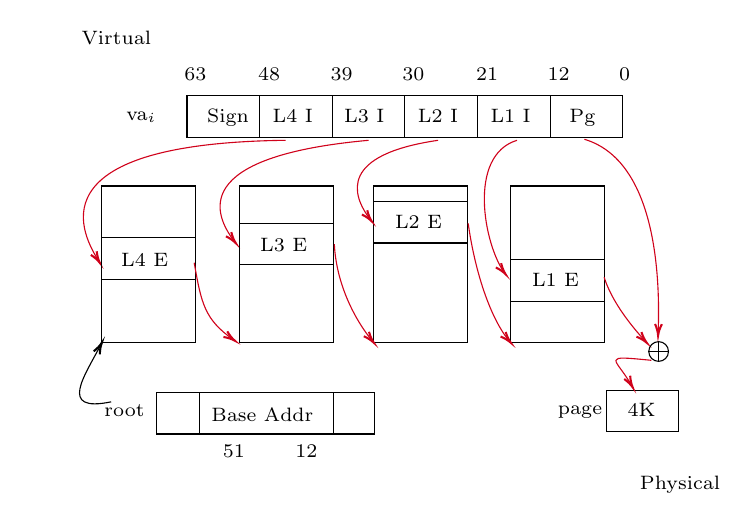
\begin{tikzpicture}[x=0.75pt,y=0.75pt,yscale=-0.5,xscale=0.5]
%uncomment if require: \path (0,471); %set diagram left start at 0, and has height of 471

%Shape: Rectangle [id:dp6797306099675045] 
\draw   (34,165) -- (124,165) -- (124,316) -- (34,316) -- cycle ;
%Shape: Rectangle [id:dp6192113478200691] 
\draw   (167,165) -- (257,165) -- (257,316) -- (167,316) -- cycle ;
%Shape: Rectangle [id:dp046479372017499854] 
\draw   (296,165) -- (386,165) -- (386,316) -- (296,316) -- cycle ;
%Shape: Rectangle [id:dp1806612887251846] 
\draw   (428,165) -- (518,165) -- (518,316) -- (428,316) -- cycle ;
%Shape: Rectangle [id:dp16201905390239735] 
\draw   (116,78) -- (186,78) -- (186,118) -- (116,118) -- cycle ;
%Shape: Rectangle [id:dp46359313115432044] 
\draw   (186,78) -- (256,78) -- (256,118) -- (186,118) -- cycle ;
%Shape: Rectangle [id:dp8986469180554777] 
\draw   (256,78) -- (326,78) -- (326,118) -- (256,118) -- cycle ;
%Shape: Rectangle [id:dp3960250568381902] 
\draw   (326,78) -- (396,78) -- (396,118) -- (326,118) -- cycle ;
%Shape: Rectangle [id:dp76786771788994] 
\draw   (396,78) -- (466,78) -- (466,118) -- (396,118) -- cycle ;
%Shape: Rectangle [id:dp9070245370995538] 
\draw   (466,78) -- (536,78) -- (536,118) -- (466,118) -- cycle ;
%Curve Lines [id:da6951218383977624] 
\draw [color={rgb, 255:red, 208; green, 2; blue, 27 }  ,draw opacity=1 ]   (211,121) .. controls (-36.94,123.94) and (16.69,214.28) .. (31.17,237.65) ;
\draw [shift={(32,239)}, rotate = 238.24] [color={rgb, 255:red, 208; green, 2; blue, 27 }  ,draw opacity=1 ][line width=0.75]    (10.93,-3.29) .. controls (6.95,-1.4) and (3.31,-0.3) .. (0,0) .. controls (3.31,0.3) and (6.95,1.4) .. (10.93,3.29)   ;
%Shape: Rectangle [id:dp48687197518810277] 
\draw   (34,215) -- (124,215) -- (124,255) -- (34,255) -- cycle ;
%Curve Lines [id:da7139570096435448] 
\draw [color={rgb, 255:red, 208; green, 2; blue, 27 }  ,draw opacity=1 ]   (291,121) .. controls (117.54,136.68) and (141.92,192.7) .. (161.79,218.46) ;
\draw [shift={(163,220)}, rotate = 231.34] [color={rgb, 255:red, 208; green, 2; blue, 27 }  ,draw opacity=1 ][line width=0.75]    (10.93,-3.29) .. controls (6.95,-1.4) and (3.31,-0.3) .. (0,0) .. controls (3.31,0.3) and (6.95,1.4) .. (10.93,3.29)   ;
%Shape: Rectangle [id:dp32338125663089956] 
\draw   (167,201) -- (257,201) -- (257,241) -- (167,241) -- cycle ;
%Shape: Rectangle [id:dp6104052627034173] 
\draw   (296,180) -- (386,180) -- (386,220) -- (296,220) -- cycle ;
%Shape: Rectangle [id:dp49476345634718477] 
\draw   (428,236) -- (518,236) -- (518,276) -- (428,276) -- cycle ;
%Curve Lines [id:da3926551025530285] 
\draw [color={rgb, 255:red, 208; green, 2; blue, 27 }  ,draw opacity=1 ]   (358,121) .. controls (263.92,134.72) and (273.56,172.45) .. (292.81,197.48) ;
\draw [shift={(294,199)}, rotate = 231.34] [color={rgb, 255:red, 208; green, 2; blue, 27 }  ,draw opacity=1 ][line width=0.75]    (10.93,-3.29) .. controls (6.95,-1.4) and (3.31,-0.3) .. (0,0) .. controls (3.31,0.3) and (6.95,1.4) .. (10.93,3.29)   ;
%Curve Lines [id:da38615138851194764] 
\draw [color={rgb, 255:red, 208; green, 2; blue, 27 }  ,draw opacity=1 ]   (434,121) .. controls (385.98,135.7) and (402.31,221.47) .. (421.8,248.42) ;
\draw [shift={(423,250)}, rotate = 231.34] [color={rgb, 255:red, 208; green, 2; blue, 27 }  ,draw opacity=1 ][line width=0.75]    (10.93,-3.29) .. controls (6.95,-1.4) and (3.31,-0.3) .. (0,0) .. controls (3.31,0.3) and (6.95,1.4) .. (10.93,3.29)   ;
%Curve Lines [id:da8796700124764012] 
\draw [color={rgb, 255:red, 208; green, 2; blue, 27 }  ,draw opacity=1 ]   (499,120) .. controls (574.46,142.54) and (571.17,273.61) .. (570.06,307.07) ;
\draw [shift={(570,309)}, rotate = 271.91] [color={rgb, 255:red, 208; green, 2; blue, 27 }  ,draw opacity=1 ][line width=0.75]    (10.93,-3.29) .. controls (6.95,-1.4) and (3.31,-0.3) .. (0,0) .. controls (3.31,0.3) and (6.95,1.4) .. (10.93,3.29)   ;
%Curve Lines [id:da26463336009584704] 
\draw    (43,373) .. controls (-9.21,383.84) and (18.15,347.13) .. (33.32,317.36) ;
\draw [shift={(34,316)}, rotate = 116.57] [color={rgb, 255:red, 0; green, 0; blue, 0 }  ][line width=0.75]    (10.93,-3.29) .. controls (6.95,-1.4) and (3.31,-0.3) .. (0,0) .. controls (3.31,0.3) and (6.95,1.4) .. (10.93,3.29)   ;
%Curve Lines [id:da18202057955172246] 
\draw [color={rgb, 255:red, 208; green, 2; blue, 27 }  ,draw opacity=1 ]   (123,239) .. controls (129.9,278.4) and (132.91,293.54) .. (160.71,313.1) ;
\draw [shift={(162,314)}, rotate = 214.59] [color={rgb, 255:red, 208; green, 2; blue, 27 }  ,draw opacity=1 ][line width=0.75]    (10.93,-3.29) .. controls (6.95,-1.4) and (3.31,-0.3) .. (0,0) .. controls (3.31,0.3) and (6.95,1.4) .. (10.93,3.29)   ;
%Curve Lines [id:da39925694981212034] 
\draw [color={rgb, 255:red, 208; green, 2; blue, 27 }  ,draw opacity=1 ]   (258,221) .. controls (259.95,260) and (278.06,294.25) .. (294.72,314.47) ;
\draw [shift={(296,316)}, rotate = 229.64] [color={rgb, 255:red, 208; green, 2; blue, 27 }  ,draw opacity=1 ][line width=0.75]    (10.93,-3.29) .. controls (6.95,-1.4) and (3.31,-0.3) .. (0,0) .. controls (3.31,0.3) and (6.95,1.4) .. (10.93,3.29)   ;
%Curve Lines [id:da0025982000064483923] 
\draw [color={rgb, 255:red, 208; green, 2; blue, 27 }  ,draw opacity=1 ]   (387,201) .. controls (393.86,250) and (409.36,294.2) .. (426.92,314.77) ;
\draw [shift={(428,316)}, rotate = 228.01] [color={rgb, 255:red, 208; green, 2; blue, 27 }  ,draw opacity=1 ][line width=0.75]    (10.93,-3.29) .. controls (6.95,-1.4) and (3.31,-0.3) .. (0,0) .. controls (3.31,0.3) and (6.95,1.4) .. (10.93,3.29)   ;
%Curve Lines [id:da4425456634879614] 
\draw [color={rgb, 255:red, 208; green, 2; blue, 27 }  ,draw opacity=1 ]   (518,253) .. controls (525.76,277.25) and (544.81,300.56) .. (557.81,314.71) ;
\draw [shift={(559,316)}, rotate = 227.12] [color={rgb, 255:red, 208; green, 2; blue, 27 }  ,draw opacity=1 ][line width=0.75]    (10.93,-3.29) .. controls (6.95,-1.4) and (3.31,-0.3) .. (0,0) .. controls (3.31,0.3) and (6.95,1.4) .. (10.93,3.29)   ;
%Shape: Rectangle [id:dp20590678105984384] 
\draw   (520,362) -- (590,362) -- (590,402) -- (520,402) -- cycle ;
%Shape: Rectangle [id:dp8145206670609288] 
\draw   (87,364) -- (128.5,364) -- (128.5,404) -- (87,404) -- cycle ;
%Shape: Rectangle [id:dp5322999267202655] 
\draw   (128.5,364) -- (257.5,364) -- (257.5,404) -- (128.5,404) -- cycle ;
%Shape: Rectangle [id:dp44035388924299834] 
\draw   (257.5,364) -- (297,364) -- (297,404) -- (257.5,404) -- cycle ;
\draw   (561,324.5) .. controls (561,319.25) and (565.25,315) .. (570.5,315) .. controls (575.75,315) and (580,319.25) .. (580,324.5) .. controls (580,329.75) and (575.75,334) .. (570.5,334) .. controls (565.25,334) and (561,329.75) .. (561,324.5) -- cycle ; \draw   (561,324.5) -- (580,324.5) ; \draw   (570.5,315) -- (570.5,334) ;
%Curve Lines [id:da7994290642535546] 
\draw [color={rgb, 255:red, 208; green, 2; blue, 27 }  ,draw opacity=1 ]   (563.5,333) .. controls (513.52,328.1) and (528.85,329.92) .. (544.54,357.29) ;
\draw [shift={(545.5,359)}, rotate = 241.11] [color={rgb, 255:red, 208; green, 2; blue, 27 }  ,draw opacity=1 ][line width=0.75]    (10.93,-3.29) .. controls (6.95,-1.4) and (3.31,-0.3) .. (0,0) .. controls (3.31,0.3) and (6.95,1.4) .. (10.93,3.29)   ;

% Text Node
\draw (12,13) node [anchor=north west][inner sep=0.75pt]   [align=left] {{\scriptsize Virtual}};
% Text Node
\draw (550,442) node [anchor=north west][inner sep=0.75pt]   [align=left] {{\scriptsize Physical}};
% Text Node
\draw (133,89) node [anchor=north west][inner sep=0.75pt]   [align=left] {{\scriptsize Sign}};
% Text Node
\draw (196,89) node [anchor=north west][inner sep=0.75pt]   [align=left] {{\scriptsize L4 I}};
% Text Node
\draw (265,89) node [anchor=north west][inner sep=0.75pt]   [align=left] {{\scriptsize L3 I}};
% Text Node
\draw (336,89) node [anchor=north west][inner sep=0.75pt]   [align=left] {{\scriptsize L2 I}};
% Text Node
\draw (406,89) node [anchor=north west][inner sep=0.75pt]   [align=left] {{\scriptsize L1 I}};
% Text Node
\draw (482,89) node [anchor=north west][inner sep=0.75pt]   [align=left] {{\scriptsize Pg}};
% Text Node
\draw (55,91) node [anchor=north west][inner sep=0.75pt]   [align=left] {{\scriptsize va$_i$}};
% Text Node
\draw (34,373) node [anchor=north west][inner sep=0.75pt]   [align=left] {{\scriptsize root}};
% Text Node
\draw (50,227) node [anchor=north west][inner sep=0.75pt]   [align=left] {{\scriptsize L4 E}};
% Text Node
\draw (184,213) node [anchor=north west][inner sep=0.75pt]   [align=left] {{\scriptsize L3 E}};
% Text Node
\draw (314,191) node [anchor=north west][inner sep=0.75pt]   [align=left] {{\scriptsize L2 E}};
% Text Node
\draw (446,247) node [anchor=north west][inner sep=0.75pt]   [align=left] {{\scriptsize L1 E}};
% Text Node
\draw (471,375) node [anchor=north west][inner sep=0.75pt]   [align=left] {{\scriptsize page}};
% Text Node
\draw (538,372) node [anchor=north west][inner sep=0.75pt]   [align=left] {{\scriptsize 4K}};
% Text Node
\draw (148,412) node [anchor=north west][inner sep=0.75pt]   [align=left] {{\scriptsize 51}};
% Text Node
\draw (218,412) node [anchor=north west][inner sep=0.75pt]   [align=left] {{\scriptsize 12}};
% Text Node
\draw (137,376) node [anchor=north west][inner sep=0.75pt]   [align=left] {{\scriptsize Base Addr}};
% Text Node
\draw (111,49) node [anchor=north west][inner sep=0.75pt]   [align=left] {{\scriptsize 63}};
% Text Node
\draw (182,49) node [anchor=north west][inner sep=0.75pt]   [align=left] {{\scriptsize 48}};
% Text Node
\draw (252,49) node [anchor=north west][inner sep=0.75pt]   [align=left] {{\scriptsize 39}};
% Text Node
\draw (321,49) node [anchor=north west][inner sep=0.75pt]   [align=left] {{\scriptsize 30}};
% Text Node
\draw (392,49) node [anchor=north west][inner sep=0.75pt]   [align=left] {{\scriptsize 21}};
% Text Node
\draw (461,49) node [anchor=north west][inner sep=0.75pt]   [align=left] {{\scriptsize 12}};
% Text Node
\draw (530,49) node [anchor=north west][inner sep=0.75pt]   [align=left] {{\scriptsize 0}};


\end{tikzpicture}
          \caption{Accessing to the Page Referenced by L1 Entry}
        \label{fig:enter-label}
    \end{subfigure}
    \vfill
    \begin{multicols}{2}
%    \begin{figure}
\begin{lstlisting}%[style=CStyleNum, basicstyle=\tiny]
static pte_t *pte_nxt_table (pte_t *entry){
 pte_t *next;
 // If not already present, try to allocate
 if (!entry->present){
  if (!pte_alloc(&next)) {
   return NULL;
  }
  entry->pfn = PTE_PFN((uintptr_t) next);
  entry->present = 1;
  } else {
   uintptr_t next_phys_addr = PTE_PFN_TO_ADDR(entry->pfn);        
   uintptr_t next_virt_addr = (uintptr_t) P2V(next_phys_addr);
   next = (pte_t *) next_virt_addr;
  }
  return next;
}
\end{lstlisting}
\columnbreak
\begin{lstlisting}
pte_t *walkpgdir(pte_t *l4, void *va){ 
 pte_t *l4_entry = &l4[L4I(va)];
 pte_t *l3 = pte_nxt_table(l4_entry);
 pte_t *l3_entry = &l3[L3I(va)];
 pte_t *l2 = pte_nxt_table(l3_entry);
 pte_t *l2_entry = &l2[L2I(va)];  
 pte_t *l1 = pte_nxt_table(l2_entry);
 pte_t *l1_entry = &l1[L1I(va)];  
 return l1_entry
}
\end{lstlisting}
%          \caption{Walking page-table tree to locate L1 entry C-source code.}
%        \label{fig:enter-label}
 %   \end{figure}
\end{multicols}
%\end{framed}
    \vspace{-2.5em}
    \caption{x86-64 page table lookups.}
    \label{fig:pagetables}
    \vspace{-1em}
\end{figure}

On the x86-64 architecture, the \textsc{MMU}'s address translation uses a sparse hierarchical set of tables:
\emph{page tables} (referring to pages of memory). As Figure \ref{fig:pagetables} (based on Figure 5-17 of the 
AMD64 architecture manual~\cite{amd64_manual_vol2}\footnote{While x86 up through its 32-bit incarnation were due to Intel,
the x86-64 architecture as a 64-bit extension to x86 was originally due to AMD. As a result, it is sometimes also referred to as the \texttt{amd64} architecture.}) shows, 
address translation proceeds by repeatedly taking designated slices of the virtual address and indexing into a table.
The final lookup in the page tables gives the base physical address of a 4KB page of physical memory, to which the low-order
bits of the accessed virtual address are added to determine the actual physical address retrieved. 
On x86-64, standard configurations use 4 levels of page tables, labelled levels 4 through 1, with lookups in the level 
1 page table resulting in the actual page of physical memory holding the requested data, and the low-order 12 bits 
being used to index into this page.\footnote{Technically levels 1--3 have explicit historical names,
but for brevity and consistency, we simply number them, in keeping with the newer 5th level.
Our formalization
only deals with 4-level page tables, but is straightforwardly extensible to 5.}  
The translation process or algorithm is sometimes referred to as a \emph{page-table walk}. 
While Figure \ref{fig:pagetables} and most of our constants (how many levels, which virtual address bits index which
table levels) are specific to the x86-64 architecture, ARMv8 (a.k.a.\ 
\texttt{aarch64}), RISC-V, and PowerPC use similar hierarchical page tables for address translation.
RISC-V's \texttt{sv48} paging configuration~\cite[\S 4.5]{riscv-privileged} and AArch64's 4-level paging configuration
both split 64-bit virtual addresses at the same points to index into the respective tables, so most of what follows
is equally applicable to those architectures (the only difference is that page table entries place control bits of write access, etc.,
in different orders).

The entries of each table are 64 bits wide, but each points to a physical address aligned to 4KB (4096 byte) boundaries, which leaves 12 bits to spare to 
control a validity bit (called the \emph{present} bit), a read-write bit (which permits write access through the entry if and only if it is set), 
and a range of additional bits which can be used to control caching, write-through, and more. This paper will only consider the present bit (0).

The page tables are managed by the OS, typically by a \emph{virtual memory manager} (VMM).\footnote{Not to be confused with Virtual 
Machine Monitor. We focus on non-hypervisor scenarios, but hardware virtualization extensions for both 
x86-64 and ARM make use of an additional set of page tables translating what a \emph{guest} considers to be its 
(virtualized) physical memory to actual physical memory. Our contributions should offer value in this scenario as well.}
Typically each process has its own 
page table, which the OS registers with the CPU by storing the (page-aligned)
physical address of the root of the page table treethe start of the L4 table) in a 
specific register (\texttt{cr3}) as part of switching to a new process. 
Using different mappings, which map only disjoint portions of physical memory (with some exceptions in the next section) 
is how the OS ensures memory isolation between processes.

If an instruction is executed that accesses a virtual address that either has no mapping, or does not have a mapping permitting 
the kind of access that was performed (e.g., the instruction was a memory write, but the relevant address range was marked read-only in
the relevant page table entry), the hardware triggers a \emph{page fault}, transferring control to a \emph{page fault handler} registered 
with the hardware by the OS, allowing it to take corrective action.
If no mapping was supposed to exist, this is a program bug (e.g., dereferencing virtual address 0 / NULL)
and the faulting program should be terminated. But this can also be used for
specialized functionality and optimizations, such as \emph{paging} (saving room in physical RAM and deferring
unnecessary IO by only reading program code from disk when it is accessed, or even swapping memory that has not
recently been accessed to disk, to read back in when a page fault indicates access).

The key pieces of VMM functionality are
adding a new page mapping (whether the mapped page contains zeros, file data, or swap data), and removing an existing 
page mapping.
While this initially sounds like relatively modest functionality whose implementation may be complicated by hardware 
subtleties, correctness of even these basic operations are actually quite intrictate.
Notably, updates to the page tables are performed as writes to memory --- \emph{which are themselves subject to address translation},
and finding the correct page table to update requires converting between physical and virtual addresses.
In the case of changing the mappings for the currently-active set of page tables, 
\emph{the OS kernel is modifying the tables involved in its
own access of the tables}.

Virtual memory concerns propagate to the OS scheduler, which deals with multiple 
address spaces, so must keep track of which virtual addresses are valid (and in what way) in which address spaces. 
Some virtual addresses are valid in only a single address space (e.g., a code address for a particular usermode 
process), while others are valid in all address spaces (e.g., kernel data structure pointers). 
The VMM must maintain some of these assumptions on behalf of the rest of the kernel, for example by guaranteeing that 
a certain range of virtual addresses (corresponding to the kernel's code and data) are valid in every address space.

\paragraph{Out of Scope: Translation Lookaside Buffers (TLBs)}
CPUs with MMUs typically have an additional \emph{translation lookaside buffer}
(TLB), to cache the (successful) results of page table walks, rather than transforming every virtual
memory access into 5 physical accesses. 
Any time a virtual address that was accessible becomes inaccessible (or has downgraded permissions),
the TLB (or at least entries in affected virtual address ranges) should be flushed.
In most kernels, this occurs in only a few well-known places, which is why existing verified kernels
\textsc{seL4}~\cite{Klein2009seL4,seL4TOCS} and \textsc{CertiKOS}~\cite{gu15,gu2016certikos} currently
trust that TLB flushes are handled correctly rather than actually modeling TLB hardware and verifying.
Eventual verification of TLB handling is a worthwhile long-term goal, but it is a challenging pursuit in its
own right. Based on others' early progress on verifying TLB operations in isolation~\cite{syeda2020formal}, we expect
it to be possible to combine this paper's insights with that support. 
Section \ref{sec:relwork} elaborates briefly on the challenges involved.
Even without TLB modeling,
our logic already enables verification of virtual memory management functionality that prior verified kernel work
either trusts completely (\textsc{seL4}, \textsc{CertiKOS}) or is incapable of reasoning about.
% Appendix \ref{apdx:tlb} gives more details on the challenges involved for the interested reader.
\looseness=-1

% \subsection{Virtual Memory Managers}
% \label{sec:backgroundonvmm}
% Most OS kernels have a component called a \emph{Virtual Memory Manager} (VMM)
% which is responsible for setting up page table mappings and for taking action when a page fault occurs. Often, a page 
% fault indicates a bug in a program --- for example, a null pointer dereference crashes a program not because the hardware
%  designates it an error, but because most OSes refuse to map the first 4K worth of virtual addresses, so dereferencing 
% \texttt{NULL} results in a page fault. In such cases, the OS will terminate the program.

% In other cases the OS uses page faults to implement specialized functionality and optimizations. A key example of this is 
% (confusingly) called \emph{paging}: saving room in physical RAM and avoiding unnecessary IO 
% by waiting until memory addresses for code are accessed 
% before copying them to RAM (in particular, saving process startup time); 
% or copying memory that has not recently been accessed to disk 
% (i.e., in a \emph{swap} file or partition) and marking those page table entries invalid so a future page fault will give 
% the OS the chance to copy the relevant data back into memory when the program tries to access it again.


% \todo[inline]{Colin says: we should chat about the paragraph below. We don't want to advertise too many
% challenges of VMM verification that we don't actually solve (or rather, we'd push them to the and of the paper
% as future work). But some of these I think we could split the difference with, for example by defining
% a variant of virtual-pointsto that allowed virtual address aliasing, but not actually verifying any code examples
% with it (just showing it's compatible with our approach).
% }
% For one, virtual addresses may \emph{alias} when more than one is mapped to the same physical memory. 
% This can occur when a process requests it (e.g., via \texttt{mmap} or \texttt{shm\_open} on UNIX-style kernels). 
% It also occurs automatically in most general-purpose kernels: while for normal programs the OS uses the MMU to isolate 
% and abstract physical memory, the kernel's own functionality is often easier to implement if the kernel can directly 
% access memory given its physical address, for example when interacting with hardware devices. For this reason, most 
% kernels contain an \emph{identity map} of all physical memory in a machine. 
% \todo[inline]{We should try defining an identity map on a whiteboard and see what breaks. If it's feasible we should
% tweak and get a definition in the paper. If not, we should cut the identity map discussion.}
% In some cases this is a literal identity map, 
% where for every virtual address $p$, interpreting $p$ as a virtual address instead will map back to $p$ as a physical 
% address. In other cases there is an offset involved, where to access physical address $p$ the kernel can access virtual
%  address $p+\mathit{offset}$. This identity map saves the kernel the performance cost of having to continually add and
%  remove transient mappings simply to briefly access a specific physical memory region. But this coexists with additional
%  virtual addresses (those used by most kernel code and data structures), in a form of virtual address aliasing. Note 
% that virtual address aliasing is both prevalent in general-purpose kernels, and violates the core assumption of most 
% memory models assumed by verified compilers like CompCert, which assume no virtual address aliasing.

% \todo[inline]{Colin says: Again, let's chat about the next paragraph. This might be another where we can
% split the difference on extension by defining something and proving a $\ast-\ast$ kind of result for sharing
% page table fragments, rather than actually proving any new code. I'm less sure about this one, though.
% }
% Another complicating factor is that portions of page tables can be shared, i.e., trees of page tables can overlap and
% become forests. 
% One common way this used to happen was for one subtree of page tables to map the kernel if linked in appropriately to 
% a higher-level page table, and then to reuse that kernel mapping portion in every process's page tables. This was mostly 
% phased out in the wake of Spectre, but remains relevant on correctly-implemented hardware.

\subsection{Separation Logic}
\label{sec:seplogic}
% \todo{Colin says: I added this b/c prior systems reviewers wanted more verification background...
% not sure how I feel about it}
Separation logic~\cite{reynolds02} is a descendant of classic Hoare logic~\cite{hoare69},
where in addition to pre- and postcondition assertions, assertions themselves pick up a
\emph{separating conjunction} operator $\ast$, such that an assertion $A\ast B$ means $A$ and $B$ are true
of disjoint pieces of state. This allows for local reasoning about updates, because it articulates
that updates to the state backing $A$ do not affect the truth of $B$. This is classically demonstrated
through the \emph{points-to} assertion: $l\mapsto v$ asserts that the memory cell at address $l$ holds value $v$:
knowing $x\mapsto 3\ast y\mapsto 4$ and writing through $x$ means information about $y$ is preserved:
$\{x\mapsto 3\ast P\}\;x\mathrel{:=}5\;\{x\mapsto 5 \ast P\}$ can be derived for any $P$.

We build on the \iris~\cite{jung2018iris} separation logic framework,
an abstract separation logic embedded in Rocq, which is useful for both metatheoretical work
and interactive correctness proofs using the logic. Given an operational
semantics structured a certain way (in our case, semantics for
a fragment of x86-64 assembly including address translation),
if a small number of ``glue'' lemmas are proven, \iris
provides a ready-made separation logic with a number of advanced features, including
higher-order ghost state and impredicative invariants, for no additional work.

We suppress many details of \iris assertions for brevity, but briefly note
a few recurring details used heavily in \iris but not necessarily in traditional
separation logics.
Because \iris is an embedded framework in \rocq, proofs in \iris-derived
logics (including ours) often encapsulate raw \rocq assertions: $\ulcorner P \urcorner$ is an embedding
of the \rocq assertion $P$ into an \iris assertion (used for things like equality and other
general pure logical assertions), similar to prior \rocq-embedded program logics~\cite{Chlipala2013Bedrock}. Newly-defined \iris assertions are in fact
\rocq terms of a particular type, rather than being drawn from a fixed vocabulary.
We introduce other details as they arise.

\iris includes two forms of implication. The magic wand operator $\wand$ is an affine implication:
$A\wand B$ describes a resource which, if combined with a resource satisfying $A$, will satisfy $B$.
Notably, this implication involves no changes to ghost state. \iris, building on the Views framework~\cite{Dinsdale-Young2013Views},
also includes a \emph{view shift} operator $\vs$ which models updates to ghost state: $A \vs B$
means resources satisfying $A$ may be transformed into resources satisfying $B$, intuitively by updating only ghost state.\footnote{\iris
experts may note that this is \emph{technically} mildly misleading given how \iris's update modalities and weakest precondition
are defined, but
this is adequate intuition for non-experts in \iris to follow their use.
}
\looseness=-1

% Of particular interest to us, \iris's machinery is largely agnostic to the particular choice of
% \emph{resource algebra}\footnote{A modern descendant of the venerable partial commutative monoid used
% to abstractly model earlier separation logics~\cite{calcagno2007local}, 
% with additions to support the step-indexing required to solve the recursive domain equations
% that arise with higher-order ghost state and impredicativity~\cite{birkedal2011step,hobor2010theory}.
% }
% used to give algebraic semantics to the connectives of the assertion language.
% This means we can drop in an alternative model that naturally supports working with respect to
% a locally-fixed context, like an address space.

% Also relevant is that \textsc{Iris} naturally decomposes the traditional Hoare triple $\{P\}\;C\;\{Q\}$
% into the precondition implying the weakest precondition of the program with respect to the postcondition ---
% $P \wand \textsf{wp}\;C\;\{v\ldotp Q\}$.\footnote{An idea with long history~\cite{pratt1976semantical}.}
% This is a natural fit for assembly-level verification, where the \emph{Hoare double}

An important limitation here is that to date, every separation logic
has assumed that all pointer addresses are meant for use in a single address space, which avoided the
problem of tracking that certain points-to assertions are true only for certain address spaces, but not others.

\subsection{Modal Logic}
\label{sec:backgroundonmodallogic}
The problem of needing to keep track of things being true in some contexts and not in others is hardly unique to virtual 
memory management, and is the general insight behind most flavors of modal logic, which use
unary operators to express that a logical claim $P$ is \emph{contingently} true 
in certain other circumstances, such as in other times~\cite{pnueli1977temporal} or places~\cite{murphy2008type,gordon2019modal}.

%   A unifying concept across any modality is that they behave as applicative functors, 
% typically satisfying (directly, or as a derived law, depending on the modality):
% \[ (P\rightarrow Q) \rightarrow M(P) \rightarrow M(Q)\]
% %\todo[inline]{Ismail, I think this means we have pure intro, $\square P \mathrel{-\ast} [r](\square P)$ if I'm using the right symbol for pure assertions }
% %\todo[inline,color=red]{The above todo comment isn't quite right.
% %Purity is about being able to duplicate. You had defined another typeclass/property-of-assertions that meant it didn't
% %care what address space it was in (like physical pointstos). That's orthogonal to purity.
% %}
% Many modalities, so-called \emph{normal} modalities also possess introduction rules of the form $P\rightarrow M(P)$, 
% the classic example being that if $P$ is true, then $P$ is \emph{necessarily} true with the contingency picked up.%($\square P$).

Of particular interest for reasoning about virtual memory are modalities that permit \emph{naming} the alternate 
circumstances, prominently \emph{hybrid} modal logics~\cite{blackburn1995hybrid,areces2001hybrid}, which come equipped 
with assertions of the form $[\ell](P)$ indicating that $P$ is true in the specific alternate circumstance (Kripke world)
 named by the \emph{nominal} $\ell$. Note that a distinctive property of hybrid logics is that, rather than hiding
the points at which a modal assertion is evaluated inside the modality's definition, the choice of what world a modalized
assertion should be true in is chosen \emph{in the assertion itself}. This allows assertions to talk about not simply whether some other assertion
is true in some possible future or past world related in a fixed way to the current world, but to talk about \emph{arbitrary}
other worlds. This explicit naming of alternate worlds increases the power of modal logics~\cite{blackburn1995hybrid}, and is actually
necessary for completeness in classical separation logics~\cite{brotherston2014parametric}.
%   A key distinguishing feature of
% hybrid logic is that the logic itself does not fix the set of modalities, but is defined relative to any set of sensible worlds.

For our purposes, these are natural candidates to adapt for virtual memory management. We can reinterpret the notion of 
naming an alternate world slightly more loosely, and instead name \emph{address spaces} by the physical address of the 
page table root, since these structures are the physical representations of page tables. Thus in this paper we develop 
the notion that we can represent contingent truth of an assertion via $[r](P)$ indicating that $P$ holds in the address 
space rooted at physical address $r$. Because OS kernels create and destroy address spaces, it is sensible to use
a hybrid-style logic that is not specialized to a fixed set of modalities, but this introduces
some subtleties from the fact that the existence of certain modalities (address spaces) can change.

% The typical hybrid modality introduction rule, that $P$ and $\ell$ (indicating the current world is $\ell$) imply 
% $[\ell](P)$, has a natural analogue: knowing $P$ and that the current address space is $r$ (i.e., that $r$ is the 
% current \texttt{cr3} value) suggests a way to construct $[r](P)$. 
% We identify an assertion as \emph{contextual} if its validity depends on the choice of address space. Used outside an explicit
% modality, the truth of this assertion depends on the current \texttt{cr3} value. Used under an explicit address space
% modality, its truth depends on both the modality-chosen address space and associated physical resources.
% \begin{itemize}
%   \item as a \textit{contextual} fact if its validity depends on \texttt{cr3} when it is outside the modality (i.e. modal context), and made 
%   \texttt{cr3} independent as a part of custom-tailored modal logic for virtual-memory: a truth representing a virtual-memory addressing depends
%    \texttt{cr3} due to address-translation operation, is dependent on \texttt{cr3} in the ambient-logic (e.g. separation-logic),
%     and is made \textit{independent} of the facts related to \texttt{cr3} by being introduced into the modal context under the assumption that
%     it exhibits the knowledge on its validity with respect to \texttt{cr3} in the ambient logic.
%   \item as a \textit{pure} fact as long as it does not \textit{necessarily} depend on any fact related to \texttt{cr3}: a truth representing a raw physical memory addressing, unlike virtual-address translation, does not need the \textit{knowledge} of \texttt{cr3}, therefore it can be introduce into the modal context as a pure fact
% \end{itemize}

Interaction of hybrid modalities and substructural reasoning is relatively unexplored (see Section \ref{sec:relwork}).
% A relatively under-explored space of modal logics is the interaction of modal and substructural logics, 
% in particular hybrid-style modalities in substructural logics, which has seen only minimal exploration~\cite{dovsen1992modal,restall1993modalities,d1997grafting,kamide2002kripke,licata2017fibrational} and no prior 
% application. 
Our development atop \iris~\cite{jung2018iris} needs to explore some additional subtleties 
that arise where the modality itself may entail ownership of resources, 
as well as interactions between our hybrid-style 
modality and substructural rules.  
% For example, Iris contains a number of modalities that distribute over separating 
% conjunction, or for which resources can freely move into the modality 
% (e.g., $\blacktriangleright(P)\ast Q \wand \blacktriangleright(P\ast Q)$). In our setting some of these rules 
% apply while others do not. For example, 
% In our setting, an assertion that involves no modalities is interpreted as 
% holding in the current (active-on-the-CPU) address space, so clearly cannot move into arbitrary other address spaces,
% while address-space-relative assertions 
% --- unless guarded by another address space modality.
Some prior \iris-based work~\cite{dang2019rustbelt,dang2022compass} has constructed derived modalities in the style we propose, indexed
by thread IDs. However in that setting, the intepretation of those modalities was fully fixed ahead of time (to refer to essentially buffers in operationalized versions of C11
concurrency). In this setting, while our modalities will be indexed by page table roots, it is possible to modify the address translation for an address
space with root $r$ --- thus changing the interpretation of a modality, and even whether a modality is valid --- \emph{while assertions with that modality are active}.
%
%
%Work on modal logic extends back for decades with many widely-varied variations; we discuss here only the pieces most relevant to our work.
%Broadly speaking modal logics incorporate \emph{modal operators}, which take as arguments a proposition expected to be true in another time~\cite{pnueli1977temporal}, place~\cite{gordon2019modal}\todo{other cites}, or circumstance~\cite{hintikka1962knowledge,halpern1985guide}, and result in a proposition true in the \emph{current} time, place, or circumstance at which the truth of the use of the modal operator is being evaluated. Classic examples include modal necessity $\square P$ describing that $P$ is \emph{necessarily} true, $\mathsf{G}~P$ meaning $P$ is true \emph{globally} (i.e., forever from this time onwards), or $K_i(P)$ describing that a particular participant $i$ \emph{knows} that $P$ is true. The latter is an example of of \emph{multimodal} logic, where there is an indexed family of modalities (modal operators) parameterized by some dimension of interest (there, participants).
%A closely related variant of multimodal logic is \emph{dynamic logic}~\cite{pratt1976semantical}, a logic of weakest preconditions~\cite{dijkstra-75} which works with modalities of the form $[p](P)$, which states that \emph{in the current program state}, \emph{if} program $p$ is run then afterwards $P$ will hold (modulo non-termination).
%This same idea is used to encode Hoare triples in the Iris program logic~\cite{krebbers2017essence}, using the same encoding as in Pratt's original presentation, where a Hoare triple $\{P\}C\{Q\}$ is encoded as $P\rightarrow[C](Q)$. Unlike classic work on dynamic logic~\cite{harel2000dynamic}, Iris applies these ideas in a \emph{substructural} setting (separation logic) where distributivity laws over substructural connectives must be considered. For both the dynamic modality and the later modality $\blacktriangleright$ used for guarded recursive predicates, these modalities satisfy axioms of the form $M(P)\ast Q\vdash M(P\ast Q)$, but not the reverse.
%Iris is not the first combination of modal and substructural logic~\cite{dovsen1992modal,restall1993modalities,d1997grafting,kamide2002kripke,licata2017fibrational}, but is certainly the most heavily tested.
%A hallmark of a unary logical operator $M$ being a modality is if $M$ satisfies an property akin to $(\upvarphi\rightarrow\psi)\rightarrow M(\upvarphi)\rightarrow\psi$, which roughly states that modus ponens holds under the modality.\footnote{Afficionados of modal logic will note that this property is not quite Axiom K (which requires the initial implication to also hold under $M$), but follows from K and a necessitation rule $\upvarphi\rightarrow M(\upvarphi)$. Non-necessitive modalities typically satisfy the weaker property we call out above.}
%Another pillar of our work is hybrid logic, a branch of modal logic with \emph{names} (called \emph{nominals} for states in Kripke models~\cite{blackburn1995hybrid,goranko1996hierarchies,areces2001hybrid,gargov1993modal}, in contrast to the typical flavor of modality which refers to an \emph{unspecified} (in the assertion) set of alternative circumstances. 
%
%Our work draws on ideas from hybrid modal logics, applied in the context of Iris's higher-order separation logic~\cite{jung2018iris}. We define our modalities and prove their rules directly within Iris, so there is no model-theoretic novelty in our work. Instead, we show that targeted use of modalities combining the ideas of \emph{named resources} with the power of substructural reasoning enable clear specification of general reasoning principles for data structures. Along the way we take advantage of the fact that modalities need not be injections between the \emph{same} logics, but in fact the propositions that modal operators contextualize can come from \emph{other} logics; in our case we exploit the fact that Iris itself is parameterized by a choice of step-indexed~\cite{ahmed-appel-virga-02} \textsf{BI}-algebra~\cite{ohearn1999bunched} to allow convenient specifications in embedded data-structure-relative logics.

\section{Syntax: Sequencing \& Executing Instructions}
\label{sec:syntax}
In this paper, we introduce a simple language for createing a stream of instructions and executing a single one to change the machine state.
\begin{figure}[!ht]
\newcommand{\commentary}[1]{ & \text{\small\it #1} \\}
\[
  \begin{array}{r@{\;}c@{\;}l}
    \loc & \in & \Loc \\
    \val & ::= & \vunit

\\
    \instrs & ::= &
    \begin{array}[t]{@{}l@{\hspace{10mm}}l@{}}
    \begin{array}[t]{@{}ll@{}}
      \iskip
                   \commentary{no-op}
      \iseq\instr\instrs
                   \commentary{sequencing}
      \ising\instr
                   \commentary{executing}             
    \end{array}
    %&
    %\begin{array}[t]{@{}ll@{}}
     % \ialloc\lval\allocsize
      %             \commentary{heap allocation}
    %\end{array}
    \end{array}
    \\

    \ectx & ::= &
      \hole \mid
      \iseq\ectx\instrs 
    \\
  \end{array}
\]
\caption{Syntax}
\Description{Syntax}
\label{fig:syntax}
\end{figure}



\section{Semantics}
\label{sec:semantics}
\subsection{State}
\label{sec:state}
We represent the machine state mainly as a finite map of registers to register values and a map of masked physical memory addresses to 64-bit physical memory values. Together with default def\textsf{CPU} instantiation, we end up having our state with following pieces:
\begin{itemize}
\item A constant cpu initialized with default value: $\sigma.\mathcal{C}$
\item A register map: $\sigma.\mathcal{R}: \kw{greg} \rightarrow_{\textrm{fin}} \kw{regval} $
\item A memory map: $\sigma.\mathcal{M}: \Locft \rightharpoonup_{\textrm{fin}} (\Loctw \rightharpoonup_{\textrm{fin}} \Locsf )$
\end{itemize}
\subsection{Indexed Memory \& Register by References}
\label{sec:}
As one might have already anticipated from the syntax we introduce, we do not bind any value of an evaluated expression. All the indices and accessed values are treated as globally referenced. In align with this design choice, our expression is a stream of instructions, which is not evaluated to a value to be bound, but changes the machine state through the indices (e.g. $\kw{r}\in\kw{greg}$) -- to the global maps. 
\subsection{Instructions}
\label{sec:instrsemantics}
The syntax of instructions is given in \fref{fig:syntax}. Their
small-step operational semantics, a~reduction relation of the form
$\hsfork{\instr}{\store}{\instr'}{\store'}{\instrs}$,
is defined in \fref{fig:semantics}.
%
The last argument~$\instrs$ is a list of newly-spawned threads;
when it is empty, we omit it
and write just $\hs{\instr}{\store}{\instr'}{\store'}$.
\subsection{A Set of Selected Instructions Changing the Machine State}
\label{sec:selectedinstrsemantics}
In addition to the reduction rules in Figure \fref{fig:reductionsemantics} for the light-weight integration of our machine model to our simple language, and, finally, to our reasoning principles, we think that it is worth building the intuition on the way some of the instructions -- specifically the ones used in the examples contained in this paper -- change the machine state when reduced with \RULE{StepContext}. \RULE{StepMovRR} in \fref{fig:instrsemantics} shows how machine state change when we copy the source register's value ($\rvsrc$) referenced by the register name ($\rgsrc$) to the destination register ($\rgdst$). We follow the convention of showing only the pieces of the machine state changed after the instruction execution -- only the register value of the destiantion register ($ \readlval\rgdst\storeregprime\rvsrc$) has changed in the state ($\storeprime$) after the execution of the instruction $\textsf{mvrr}$. All the other rules in Figure \fref{fig:instrsemantics}, presents the change in the state when a value is loaded/stored to/from register/memory, and are differentiated with respect to the addressing mode ($amode$) which determines whether the accessed memory address is computed based on some offset (\RULE{StepMovRMOff}, \RULE{StepMovMROff}) or not (\RULE{StepMovRMBase}) and \RULE{StepMovMRBase}). The most common essential aspect of loading the source register's value ($\rvsrc$) to the memory, \RULE{StepMovRMBase} and \RULE{StepMovRMOff}, is the hierarchical translation of memory location, $\readlval{\plusaddr\maddr\offs}{\storememstar\crval}\locsf$, which is hidden in the rules, expanded as the following:
\begin{itemize}
\item
\item
\item
\item
\end{itemize}
where the first three levels of translation allows address-translation .
\begin{figure}[!ht]
\small
\begin{mathpar}
\inferrule[StepSeqSkip]{}{
  \hsnostore{\iseq\iskip\instr}{\instr}
}
\inferrule[StepContext]{
  \hsforknl{\instr}{\store}{\instr'}{\store'}{\instrs}
}{
  \hsforknl{\efill\ectx\instr}{\store}{\efill\ectx{\instr'}}{\store'}{\instrs}
}
\end{mathpar}
\caption{Small-Step Operational Reduction Rules for Light-Weight Integration of \textsf{AMD64} Machine Model}
\label{fig:reductionsemantics}
\end{figure}

\begin{figure*}[!ht]
  \small
  \begin{mathpar}
\inferrule[StepMovRR]{
  \readlval\rgsrc\storereg\rvsrc \\\\
  \readlval\rgdst\storereg\rvdst\\\\
  \readlval\rgsrc\storeregprime\rvsrc \\\\
  \readlval\rgdst\storeregprime\rvsrc
}{
  \hs{\imov \mvrr \rgsrc\rgdst}\store
     \iskip{\store'}
}\qquad
\inferrule[StepMovRMOff]{
  \amodeo\imreg \; \readlval\rgsrc\storereg\rvsrc \\\\
   \readlval\imreg\storeregprime\maddr \; \readlval\imreg\storereg\maddr \\\\
     \readlval\rgsrc\storeregprime\rvsrc  \\\\
          \readlval{\plusaddr\maddr\offs}{\storememstar\crval}\locsf \\\\
         \readlval{\plusaddr\maddr\offs}{\storememprimestar\crval}\rvsrc
}{
  \hs{\imov\mvrmo\rgsrc\amode}\store
     \iskip{\store'}
}\qquad
\inferrule[StepMovRMBase]{
  \amodeb\imreg \; \readlval\rgsrc\storereg\rvsrc \\\\
   \readlval\imreg\storeregprime\maddr \; \readlval\imreg\storereg\maddr \\\\
     \readlval\rgsrc\storeregprime\rvsrc  \\\\
     \readlval\maddr{\storememstar\crval}\locsf \\\\
      \readlval\maddr{\storememprimestar\crval}\rvsrc
}{
  \hs{\imov\mvrmb\rgsrc\amode}\store
     \iskip{\store'}
}\\
\inferrule[StepMovMROff]{
  \amodeo\imreg \; \readlval\rgsrc\storereg\rvsrc \\\\
   \readlval\imreg\storeregprime\maddr \; \readlval\imreg\storereg\maddr \\\\
     \readlval\rgsrc\storeregprime\locsf  \\\\
          \readlval{\plusaddr\maddr\offs}{\storememstar\crval}\locsf \\\\
         \readlval{\plusaddr\maddr\offs}{\storememprimestar\crval}\locsf
}{
  \hs{\imov\mvmro\amode\rgsrc}\store
     \iskip{\store'}
}\qquad
\inferrule[StepMovMRBase]{
  \amodeb\imreg \; \readlval\rgsrc\storereg\rvsrc \\\\
   \readlval\imreg\storeregprime\maddr \; \readlval\imreg\storereg\maddr \\\\
     \readlval\rgsrc\storeregprime\locsf  \\\\
          \readlval{\plusaddr\maddr\offs}{\storememstar\crval}\locsf \\\\
         \readlval{\plusaddr\maddr\offs}{\storememprimestar\crval}\locsf
}{
  \hs{\imov\mvmro\amode\rgsrc}\store
     \iskip{\store'}
}
\end{mathpar}
\caption{Small-Step Relations for Chosen Instructions in \textsf{AMD64} Model}
\Description{Small-Step Relations for Chosen Instructions in \textsf{AMD64} Model}
\label{fig:instrsemantics}
\end{figure*}


\section{Program Logic for Location Virtualization}
\label{sec:logic}
Our reasoning principles are shaped around understanding the following issues exhibiting themselves withing the context of vritual-memory-management:
\begin{enumerate}
\item abstracting the relation between memory (virtual) addresses and the physical page addresses backing these virtual addresses
\item regarding the address-space management, we propose reasoning principles for
  \begin{itemize}
  \item aliasing/sharing Physical Pages:
  \item abstracting address-space as a modality
    \begin{itemize}
    \item modal resource context:
    \item interaction:
    \end{itemize}
    \item Hoare-Doubles: 
  \end{itemize}
\end{enumerate}
%\subsection{Machine State under Address Translation}
%\label{sec:selectedinstrsemantics}
%Althought we give the complete set of operational semantics rule in \sref{appendix:movops}, It is worth building the intuition on the the way some of these rules bahave in the context of address translation. In fact $\readlval\maddr{\storememstar\crval}\locsf$ is unfoled into multiple physical memory lookups for the final page address retrieval -- i.e. address translation traversal as shown in Figure \ref{fig:pagetables}:
%\begin{itemize}
%\item top-level-address translation: with the given root address (64-bit $\crval$) of the address space, performs the address translation, handling the first level (to get the PML4 entry) itself. The next level table address is computed with the fetched PML4 offset value which exhibits itself as 9-bit offset in $\kw{maddr}$. \mytodo{iso: put move}
%\item translating from PML4 entry: performs the second level of address translation, to retrieve starting at the PML4 table entry, and interprets the PML4 entry that references a Page-Directory-Pointer Table (PDPT). We obtain the PDPT offset which exhibits itself as 9 bit offset in $\kw{maddr}$ to obtain the address of the next level page directory table (PDT) \mytodo{iso: put move}
%\item translating from PD entry: performs the third level of address translation, to retrieve starting at the PDP table entry, and interprets a PDPTE that references a PD table. Likewise, we obtain the PD offset which exhibits itself as 9 bit offset in $\kw{maddr}$ to obtain the address of the next level page directory table (PT) \mytodo{iso:put move }
%\item translate from PT entry: performs final level of address translation, starting from the PT entry, with a given 12 bit page offset, we can compute the physical address referencing $\locsf$ \mytodo{ismo: put mov}
%\end{itemize}
\subsection{Points-To Assertions}
\label{sec:pointsto}
As part of assertions on our machine state ($\sigma$), we abstract memory addresses and registers naming their relevant values through well-known separation logic assertion \textit{points-to}.
\begin{enumerate}
\item Physical address points-to, $\pfpointsto\locsf\locsf\qfrac\ppts$
\item Register points-to, $\pfpointsto\rg\rv\qfrac\rpts$
\end{enumerate}
\paragraph{Register points-to} The assertion $\pfpointsto\rg\rv\rpts\qfrac$ ensures the ownership of the register $\rg$ naming the register value $\rv$. The fraction $\qfrac$ with value 1 asserts the unique ownership of the register mapping, and grants update permission on it, otherwise, any value $0 < \qfrac <1$ represents partial ownership granting readonly permission on the mapping.
\paragraph{Physical-Memory points-to} The our physical memory points-to relation ($\pfpointsto\locsf\locsf\qfrac\ppts$) exhibits nested-mappings due to masking applied on the indexing address ($\locsf$). The unfolded definition of the physical mapsto 
\begin{figure}[!ht]
\[
\begin{array}{cl}
\pfpointsto\locsf\locsf\qfrac\ppts \stackrel{def}{=} & \nfpointsto{\mask\locsf\ft}{\mask\locsf\tw}\locsf\qfrac\naddr
\end{array}
\]
\caption{Physical Points-to with Nested Masking}
  \label{fig:physicalpointsto}
\end{figure}
where we simply abstract the generation of hierarchical mapping of a physical address ($\locsf$) through two different levels of masking:

\begin{itemize}
\item  After a series of masking imposed on the virtual memory address (e.g. \textsf{vaddr} 64bits address [0-64]) :
  \begin{itemize}
  \item Page Map Level-4 Translation (L4): Calculating the offset to the 4 \textsf{Kbyte Physical Page} table to obtain the  physical address by  which resides in the last 12 bits of the virtual memory address, $\locsf|^{12}$,  shown in Figure \ref{}.  
  \item Page Directory Pointer Level Translation (L3):
  \item Page Directory Table Level Translation (L2):  we obtain the address of the page table via \textsf{PDE}$|^{52}$ and picking the offset from the virtual memory address via imposing the mask to obtain page table offset bits (9 bits [20-12] shown in Figure \ref{}) to obtain the page table entry (\textsf{PTE}).
  \item Page Table Level Translation (L1): 
  \end{itemize}
 \item then after obtainini the physical page address, we obtain the value 
\end{itemize}


\paragraph{Virtual-Memory points-to} As we see in Figure \fref{fig:}, virtual address mapping is obtained via traversal of page table, i.e. indirection provided by physical memory lookups. As expected, we define the virtual-points to relation, ($\pfpointsto\vaddr\locsf\qfrac\vpts$), in terms of multiple physical memory mappings representing the indirection shown in Figure \fref{fig:}
\begin{figure*}
\[
\begin{array}{l}
  \ppointsto\vaddr\locsf\vpts \stackrel{def}{=} \lambda \tlf\Loc.\\
  \exists_{\tlfoff\Locn \;, \tltoff\Locn \;, \tltwoff\Locn \;,\tlooff\Locn \;, \tpgoff\Loctw \;, \tlt\Loc \;, \tltw\Loc \;, \tlo\Loc \tpg\Loc} \ldotp \\
  \ulcorner \textsf{aligned } \vaddr \urcorner \star 
   \ulcorner \vaddr = \locsx :: \lfoff :: \ltoff :: 
   \ltwoff :: \looff :: \pgoff \urcorner \star\\
  \pfpointsto{\lvlsum\crt\lfoff}{\lvlbor\lt}\qfracfotsss\ppts \star 
  \pfpointsto{\lvlsum\lt\ltoff}{\lvlbor\ltw}\qfracfotss\ppts \star \\
  \pfpointsto{\lvlsum\ltw\ltwoff}{\lvlbor\lo}\qfracfots\ppts \star 
  \pfpointsto{\lvlsum\lo\looff}{\lvlbor\pg}\qfracfot\ppts \star \\
  \ppointsto{\pageptstosum\pg\pgoff}\locsf\ppts 
\end{array}
\]
\caption{Virtual Points-to Relation}
\todo[inline]{These fractions aren't quite right (though I see you added the variance between levels), I can walk you through in our meeting tomorrow.}
  \label{fig:virtualpointsto}
\end{figure*}
\subsection{Considering Hoare Doubles in the Context of Switching Address-Space}
An important subtlety arises with supporting \lstinline|mov|s into \lstinline|%cr3|. Consider the hypothetical rule:
\begin{mathpar}
\inferrule[Broken]{ }{
  \{P \ast cr3=r_1 \ast r=r_2 \ast [r_2](Q)\}
  \texttt{mov}~\texttt{\%cr3},~r%\lstinline|mov %cr3, r| 
  \{[r_1](P) \ast cr3=r_2 \ast r = r_2 \ast Q\}
}
\end{mathpar}
This rule captures the intuitive change of address space in a Hoare triple, rather than double, form. The problem with this is that it interacts quite poorly with the traditional frame rule and the modal flavor of virtual points-to assertions:
\begin{mathpar}
  \inferrule*[right=Frame]{
    \inferrule*[right=Broken]{ }{
    \{\mathsf{emp} \ast cr3=r_1 \ast r=r_2 \ast [r_2](Q)\}
    \texttt{mov}~\texttt{\%cr3},~r%\lstinline|mov %cr3, r| 
    \{[r_1](\mathsf{emp}) \ast cr3=r_1 \ast r=r_2 \ast Q\}
    }
  }{
    \{a\mapsto_\mathsf{v} x \ast \mathsf{emp} \ast cr3=r_1 \ast r=r_2 \ast [r_2](Q)\}
    \texttt{mov}~\texttt{\%cr3},~r%\lstinline|mov %cr3, r| 
    \{a\mapsto_\mathsf{v} x \ast [r_1](\mathsf{emp}) \ast cr3=r_1 \ast r=r_2 \ast Q\}
  }
\end{mathpar}
Notice that both the precondition and postcondition assert that $a\mapsto_\mathsf{v} x$ in the current address space, but we have no basis for concluding that address translation is preserved by the change of address space. So this derivation clearly leads to an unsound conclusion. This suggestss that the traditional frame rule and the Hoare triple presentation of the change-of-address-space rule cannot soundly coexist in the same system.
The heart of the problem is that while updating \lstinline|cr3| is \emph{physically} local, it globally changes the interpretation of virtual addresses. So it is simply unsound to frame around \lstinline|cr3| updates.

Switching to Hoare doubles resolves this problem because an under-appreciated subtlety of Hoare doubles is that typically \emph{there is no frame rule}. Instead each verification essentially includes a local frame that it passes to the next instructions (think continuation-passing style), giving each overall rule a \emph{global} (rather than local) precondition. For most rules this is not that important, but it does permit rules that have global effects on their preconditions.

This is then how we justify our actual rule for \lstinline|cr3| updates:
\begin{mathpar}
\inferrule[ChangeAddressSpace]{
  \{[r_1](P) \ast cr3=r_2 \ast r = r_2 \ast Q\}\overline{is}
}{
  \{P \ast cr3=r_1 \ast r=r_2 \ast [r_2](Q)\}
  \texttt{mov}~\texttt{\%cr3},~r;\;\overline{is}
  %\lstinline|mov %cr3, r| 
}
\end{mathpar}
Because the precondition on this rule is global, we avoid issues with framing.

If we wanted to consider a frame rule that would work for this logic, we could consider:
\begin{mathpar}
  \inferrule[Cr3Frame]{
    \{P\ast cr3=v\}\;C\;\{ Q \ast cr3=v\}
  }{
    \{R\ast P\ast cr3=v\}\;C\;\{ R \ast Q \ast cr3=v\}
  }
\end{mathpar}
By demanding that \lstinline|cr3| be held constant (or rather, at least restored to its original value) we could frame almost traditionally. In particular, this rule would work with framing around calls that might lead to address space switches, such as calling blocking operations in the kernel.

Readers familiar with dynamic frames~\cite{parkinson2011relationship} might find it useful to notice that a different perspective on this matter is that virtual points-to assertions are self-stable \emph{except} for changes in \lstinline|cr3|, so framing would then naturally require other means of holding \lstinline|cr3| constant (or saving and restoring it).
Virtual points-to assertions could be made self-stable by also giving them partial ownership over \lstinline|cr3| assertions, but this would require explicitly plumbing that ownership from \emph{all} assertions back to any place an address space change might occur; this would seem to be a far graver loss of modularity than this extra quirk in framing discussions.

\section{Implementing Logical Machinery \& Soundness}
We build our program logic, as an instantiation of Iris~\cite{iris}, and build our modal abstractions on top of it. 
\mytodo{we should put some stuff here}
\subsection{Soundness}
\label{sec:soundness}
Our logic, operates on the machine state, which means we do not need to augment the machine state. The invarian that we pick, \textit{central invariant} ($\mathcal{I}$\textsf{ASpace}), is just semantic interpretation of stores in the machine state, $\sigma$.R and $\sigma$.M. This semantic interpratation ensures the correct lifting of mappings in the machine state to the assertions that the client of our logic uses, i.e. points-to assertions that are defined as the ownership of a fragment of the logical state.

We prefer to skip explaining the steps used in instantiation of Iris because it is an almost standard procedure, has already been explained for many other logic \ref{}, and we are concerned with the page-count limitation. However, it is worh noting that once you instantiate Iris for your language, it comes with the semantic definition for the weakest-precondition which we can refactor into Hoare triples, $\triple\pre\instr\post$, to specify our  selected \textsf{AMD64} instructions shown in Figure \ref{fig:wpdamd}, and show that these triples are sound. 
\subsection{The Soundness Statement}
\label{def:soundness:statement}
The operational semantics of our simple lang just executes sequences of instructions in our x86-64 model. Therefore, our soundness argument is to show that any execution composed of instructions in our machine model (some of which are shown in Figure \sref{sec:semantics}) does not end-up in a invalid state.
\begin{figure*}
\small
\begin{mathpar}
\inferrule[Skip]{}{
  \triple\post\iskip\post
}

\inferrule[Seq]{
  \triple\pre{\instr_1}\midpoint \\
  \triple\midpoint{\instr_2}\post
}{
  \triple\pre{(\iseq{\instr_1}{\instr_2})}\post
}
\end{mathpar}
\caption{Structural Rules for Executing Instructions}
\Description{Reasoning Rules}
\label{fig:structural}
\end{figure*}

\begin{theorem}[Soundness of the Logic]
  \label{th:adequacy}
 Together with the assumptions on the initial state hold,
 the execution of the instruction~$\instrs$, beginning with this initial state, cannot result in a configuration where the execution is stuck.
\end{theorem}
which states that if the program~$\instr$, with the given \textsf{valid\_init} asserting a valid state initialization, satisfies a semantic Hoare
triple, then this program cannot crash: by a direct consequence of Iris's adequacy theorem~\cite[\S6.4]{iris}.

Moreover we need to show the validity of each rules in Figures \fref{fig:reasoning} and \fref{fig:laws}.
\begin{theorem}[Validity of the Reasoning Rules]
\label{th:validity}
  Each of the rules in Figures~\ref{fig:wpdamd}
  and~\ref{fig:structural} is valid.
\end{theorem}
Due to the space limits in this paper, we do not mention each proof for the rules in Figures \ref{fig:wpdamd} and \ref{fig:structural} within this section, but we provide mechanized proofs for all these in Coq as a part of our artifact submission.
However, we would like to give the definitions and constructions used in our proofs, and would like to give an outline of paper proof for \TirNameStyle{WriteToRegFromVirtMem} in Figure \ref{fig:wpdamd} within this section.

Together, Theorems~\ref{th:adequacy} and~\ref{th:validity} guarantee that, if
the Hoare triple $\textsf{valid\_init }\instrs\;\iTrue$ can be obtained by applying
the reasoning rules of our logic, then the program~$\instrs$ is safe.

\subsection{Logical Constructions}
\label{sec:invariant}
We already have the physical and logical stores and a simple invariant between them. Now, we can rely on the following Assumption \ref{assumption} from Iris to utilize its logical constructions.
% The predicate gen_heap_interp.
\newcommand{\genheapinterp}[1]{\mathit{Heap}\;#1}
\newcommand{\genmemheapinterp}[1]{\mathit{MemHeap}\;#1}
% Our predicate pred (defined in ph.v), expanded.
\newcommand{\pred}[1]{\ownGhost\gammaPred{\authfull{(\mapone\predstore)}}}
% A notation for assigning fraction 1 to every element of \predstore.
\newcommand{\mapone}[1]{1.#1}
% The predicate mapsfrom_exact, expanded.
\newcommand{\mapsfromexact}[3]{
  \ownGhost\gammaPred{\authfrag{\singletonMap{#1}{(#2, #3)}}}
}
% A metavariable for a share.
\newcommand{\sh}{L'}
% The predicate mapsfrom, expanded.
\newcommand{\mapsfromdef}[3]{
  \exists\sh.\;
  \mapsfromexact{#1}{#2}{\sh} \star \pure{\sh \subseteq #3}
}

\begin{assumption}
\label{assumption}
Iris defines two pieces of ghost state
\begin{enumerate}
\item  defines a predicate $\textsf{to\_gen\_heap }\store.\mathcal{R}$
  that ties a store~$\store.\mathcal{R}$ to this ghost state,
  and defines the points-to assertion $\ppointsto\rg\rv\qfrac\rpts$
  in terms of this ghost state.
  This is visible in the paper~\cite[\S6.3.2]{iris}
  and in Iris's \texttt{gen\_heap} library~\cite{genheap}.
  %
  We re-use this machinery without change,
  so we do not repeat these definitions.
  We mention the predicate $\genheapinterp\!$
  in our own invariant (Definition~\ref{def:invariant}),
  where it is applied to the \logical store~$\store$.
\item unlike the register points-to relation obtained by direct interpretion of $\textsf{to\_gen\_heap }\store.\mathcal{R}$ using Iris, the existing \textsf{gen\_heap\_heap},
  does not directly helps introducing the ghost we define a new algebra (\textsf{gen\_mem\_UR}) for abstracting the nested maps due to different levels of masking in memory mappings and an interpretation for this algebra. 
\end{enumerate}
\end{assumption}

\begin{definition}[Ghost State - Memory with Nested Mappings]
We define our custom-tailored algebra 
\newcommand\fpfn{\rightarrow_{\textrm{fin}}}
\( \textsf{gen\_memUR} \stackrel{def}{=}
  \authm(\;
  \Locft \;\fpfn\;
  (\Loctw \;\fpfn\;  (\textsc{Frac }, \mathord{+}) \times (\textsc{Agree } \Loc,\mathord{=}) )
  \)
  for our nested memory mapping abstracting two different machine word masking. Then, we register our \emph{authoritative camera} \cite[\S6.3.3]{iris} from this algebra
  \[\textsf{inG } \Sigma \textsf{ gen\_memUR} \]
  To interpret this nested ghost map we define \textsf{to\_gen\_mem}
  \[
  \begin{array}{l}
    \mathsf{to\_gen\_mem} : \textsf{ gmap L1 }(\textsf{gmap L2 V})\rightarrow \textsf{gen\_memUR L1 L2 V } := \textsf{ fmap} (\lambda \textsf{m . to\_gen\_heap m}). \\
     \mathsf{to\_gen\_heap } : \textsf{gmap L V} \rightarrow \textsf{gen\_heapUR L V} :=  (\lambda \textsf{v }\ldotp (1, \textsf{ to\_agree } (\textsf{v} : \textsf{leibnizO V}))).
  \end{array}
  \]
 throuh using \textsf{to\_gen\_heap} from previous Iris version. \todo[inline,color=red]{Ismail give exact version commit etc.}
As a final step, we allocate an empty ghost cell $\gamma$ at the beggining of a program execution to store the element of the monoid $\textsf{inG } \Sigma \textsf{ gen\_memUR}$.
\end{definition}

\begin{definition}[Ghost State - Register Mappings]
We allocate $\theta$ ghost cell which stores an
element of the monoid 
\newcommand\fpfn{\rightarrow_{\textrm{fin}}}
\(
  \authm(\;
    \regset \;\fpfn\;
    (\textsc{Frac}, \mathord{+})
    \times
    (\regvaltype, \mathord{=})
  \;)
\)
% \emph{authoritative camera}
\cite[\S6.3.3]{iris}.
\end{definition}

\begin{definition}[Central Invariant]
\label{def:invariant}
The central invariant of our logic is, due to lack of need for augmenting the machine state, simply the state interpretation: 
\[
\textsf{x64\_h}\;\store \triangleq
\left\{
\def\arraystretch{1.2}
\begin{array}{l@{\quad\star\quad}l@{\quad}l}
  \textsf{to\_gen\_heap} \;\store.\mathcal{R} &  \\
   \textsf{to\_gen\_mem} \; \store.\mathcal{M}
\end{array}
\right.
\]
\end{definition}

As a last definition, we give the head step relation required for the Iris instantiation for our simple language in Figure \ref{} to sequence instructions. This relation allows lifting the program expression to enables the application of changes imposed by the operational semantics on the program state $\sigma$ when applied for an insturction (\textsf{i}).
\[
\begin{array}{l}
\textsf{exec\_step} (\textsf{i}: \textsf{ instr}) (\sigma:\textsf{ state}):\textsf{ option state} \stackrel{def}{=} \\
\qquad \textsf{exec\_state} (\textsf{exec\_instr i } \sigma.(\textsf{cpu})  \\ \qquad (\textsf{regToregset } \sigma.(\mathcal{R}))  \\ \qquad ((\textsf{memToPhysMem }\sigma.(\mathcal{M})) (\textsf{exist \_}  \\ \qquad (\textsf{ regset\_get\_num }(\textsf{regToregset }\sigma.(\mathcal{R}))  (\textsf{ cr cr3}))))).
\end{array}
\]
\todo[inline,color=yellow]{Colin, in case needed,not proven, could you simply say that we assume these map equalities or a paper proof etc.}. Since the focus of this paper is not explaining our \textsf{AMD64} model, we prefer not to get into the details due to space limits. However, Coq formalization of our operational semantics is a part of our submission artifact.

Now, we have well-enough definition for giving an outline for the proof of \TirNameStyle{WriteToRegFromVirtMem}.
 \begin{lemma}[\textsc{\TirNameStyle{WriteToRegFromVirtMem}}]
   \label{lemma:unlink}
\begin{align*}
\inferrule{
  \{P \ast r_d \mapsto_{r}  \textsf{v} \ast r_a \mapsto_{r} \{q\} \textsf{ vaddr} \ast \textsf{vaddr} \mapsto_{\textsf{v,rtv}} \textsf{v} \}\;\overline{is}
}{
  \{P \ast r_d \mapsto_{r}  \textsf{rvd} \ast r_a \mapsto_{r} \{q\} \textsf{ vaddr} \ast \textsf{vaddr} \mapsto_{\textsf{v,rtv}} \textsf{v} \}
  \textsf{mov}~\textsf{r}_d,~\textsf{r}_a;\;\overline{is}
}
\end{align*}
 \end{lemma}
 
 \begin{proof}
   Assuming the inference rule realized with \textsf{wpd\_def}, we expand the precondition with $\textsf{cr3} \mapsto_{\textsf{r}} \rtv$.
   Then we do two proofs, one for head reducibility of atomic step \textsf{mov\_reg64\_mem64}, the second one for the executing the expression and obtaining the new state. Steps taken in the first one are subset of the second one, so we outline the second portion of the proof, but in case of an interest in details of the proof, Coq artifact can be consulted.

   \begin{itemize}
   \item Step 1: we apply the head step relation and obtain the current valid state $\sigma1$ interpretation : $\textsf{x64\_h}\;\store$
   \item Step 2: we unfold the virtual-pointsto ($\vaddr \mapsto_{\textsf{v,rtv}} \textsf{v}$) definition, and for an existential physical page address $\paddr$, we exchange our fragmental toke ($\sumwalkabs\vaddr\qfrac\paddr$) to obtain physical table-pointsto ($\textsf{L}_{4}\_\textsf{L}_{1}\_\textsf{PointsTo}$ in Figure \ref{fig:strongvirtualpointsto}) relation
   \item Step 3: for each physical pointsto inside $\textsf{L}_{4}\_\textsf{L}_{1}\_\textsf{PointsTo}$, we obtain
\[
       \ulcorner \sigma.\mathcal{M } !! (\textsf{ va}|^{52}(\textsf{ent}_i) = \textsf{Some } \sigma\textsf{d}_i \land
       \sigma\textsf{d }_i !! (\textsf{ va}|^{12}(\textsf{ent}_i)  = \textsf{Some entry}_{i+1} \urcorner
       \]
       where $\sigma.\textsf{d}_i$ in type \textsf{gmap (word 12) (word 64)} for our offset mappings. 
     \item Step 4: use these concrete lookups to traverse the page tables to obtain the value \textsf{v}
     \item Step 5: do the map update the $\sigma.\mathcal{R}$ for relevant register mapping ($r_d$) with the value \textsf{v} 
   \end{itemize}
   
   \end{proof}

%$\assert{\ulcorner \mathsf{aligned maddr} \urcorner \ast \mathsf{r14} \mapsto_{\textsf{r}} \textsf{r14v} \ast \mathsf{r13} \mapsto_{\textsf{r}} \textsf{maddr} \ast \mathsf{rdi} \mapsto_{\textsf{r}} \textsf{rdiv} \ast \mathsf{rax} \mapsto_{\textsf{r}} \textsf{raxv}}$
%$\assert{\ulcorner \ptablestore !! \textsf{maddr} = \textsf{None} \urcorner \ast \ownGhost\gammaPred{\authfull{\ptableabswalk\ptablestore}} \ast \textsf{Pf}} $
\section{Experiment}
\label{sec:experiment}
To both validate and demonstrate the value of the modal approach to reasoning about virtual memory management, we study several distillations of real concerns of virtual memory managers.
Recall from Section \ref{sec:logic} that virtual points-to assertions work just like regular points-to assertions, by design.

%\begin{comment}
%\todo[inline]{Identity mappings are difficult, and our current approach won't quite work. Consider trying to have a virtual pointsto for an actual page table entry (i.e., that one could use to update a page table mapping), while also having a virtual pointsto for an address that entry mapped. With the current (let's call it v1) solution, we can't actually have both of those simultaneously!  That's because the PTE pointsto will assert full ownership of the physical memory cell holding the PTE as its data value, while the virtual pointsto for the data mapped by that entry will \emph{also} assert (fractional) ownership of all entries a page table walk would traverse.
%}
%\todo[inline,color=violet]{This doesn't seem to cause issues with the mapping/unmapping examples, only with changing intermediate page table pointers. The mapping example requires a virtual pointsto for the blank PTE, and once filled in that ownership can be immediately split to create the 512 new virtual pointsto assertions for the newly mapped page. Conversely, for unmapping we'd assume ownership of all the relevant virtual pointsto assertions for the page we're unmapping, at which point we can (with a bit of work) show that they all correspond to the same L1 PTE, and extract the 512 fractional shares of that entry from the pointsto assertions.  But changing intermediate page tables, as one would do for coallescing or splitting a superpage while preserving the virtual-to-physical mappings, couldn't be done without some really complicated separating implication tricks.}
%\todo[inline,color=green]{One possible approach to resolving this, which we came up with in our Tuesday meeting, is to recognize that the current (v1) virtual points-to is too strong, because it really doesn't care about \emph{owning} those fractional resources, it only cares that \emph{something} ensures the correct page table walk exists. Iris has a ghost map resource where authoritative ownership of an individual key-value pair can be handled as a resource.  (Colin was using this in the filesystem cache.)
%We can use that mechanism to separate the virtual-to-physical translation from the physical memory involved (Kolanski and Klein may have done something similar for different reasons): (fractional) virtual points-to assertions can be defined in terms of (fractional) ownership of these authoritative ghost map entry assertions, plus sharing an invariant that the current installed page table respects all entries of the mapping. Unmapping collects the authoritative map kvpairs from collecting the assertions, and then can remove them from the ghost map and update the page tables. Critically, physical ownership of the page tables then lives in the invariant on the current page table, so some virtual pointsto assertions can refer to memory in those page tables.
%This still works with the modality, since that invariant is also semantically a predicate on a page table root.
%Let's call this v2.
%}
%\end{comment}
\subsection{Mapping a New Page}
One of the key tasks of a page fault handler in a general-purpose OS kernel is to map new pages into an address space by writing into an existing page table. To do so, we first allocate a fresh page, then calculate the appropriate known-valid page table walks and update the appropriate L1 page table entry.
\lstset{
  columns=fullflexible,
  numbers=left,
  basicstyle=\ttfamily,
  keywordstyle=\color{blue}\bfseries,
  morekeywords={mov,add,call},
  emph={rsp,rdx,rax,rbx,rbp,rsi,rdi,rcx,r8,r9,r10,r11,r12,r13,r14,r15},
  emphstyle=\color{green},
  emph={[2]cr3},
  emphstyle={[2]\color{violet}},
  morecomment=[l]{;;},
  mathescape
}
\newcommand{\fpaddr}{\texttt{fpaddr}}
\newcommand{\specline}[1]{{\color{blue}\left\{#1\right\}}}
\begin{figure}\footnotesize
  \begin{lstlisting}
$\specline{\textsf{P} \ast \mathcal{I}\texttt{ASpace}(\theta,m)  \ast  \texttt{r14}\mapsto_{r} \_ \ast \texttt{rdi}\mapsto_{r} \vaddr \ast \texttt{rax}\mapsto_{r} \_ \ast \ulcorner \texttt{aligned va} \land  \theta \; !!\; \vaddr = \texttt{None}\urcorner}_{\rtv}$
call ensure_L1_page
$\specline{\textsf{P} \ast \mathcal{I}\texttt{ASpace}(\theta,m) \ast  \texttt{r14}\mapsto_{r} \_ \ast \texttt{rdi}\mapsto_{r} \vaddr \ast \texttt{rax}\mapsto_{r} \textsf{ pte\_addr} \; \ast }_{\rtv}$
$\specline{\exists (\entryf ,\;\entrytr,\; \entrytw,\; \entryo,\;\textsf{pte\_addr },\paddr \; : \texttt{word 64}) \ldotp \ulcorner \texttt{addr\_L1 }(\vaddr, \entryo) = \paddr \urcorner \; \ast }_{\rtv}$
$\specline{\nfpointsto{\mask\vaddr\maskfour\rtv}{\mask\vaddr\maskfouroff\rtv}\entryf\qone\naddr \; \ast}_{\rtv}$ 
$\specline{  \nfpointsto{\mask\vaddr\maskthree\entryf}{\mask\vaddr\maskthreeoff\entryf}\entrytr\qtwo\naddr \ast \nfpointsto{\mask\vaddr\masktwo\entrytr}{\mask\vaddr\masktwooff\entrytr}\paddr\qthree\naddr \;\ast}_{\rtv}$
$\specline{\texttt{pte\_addr} \mapsto_{\texttt{vpte}} \paddr \;(\texttt{wzero 64}) \ast \texttt{rax}\mapsto_{r} \texttt{pte\_addr}  }_{\rtv}$
;; Returns the virtual address of the L1 entry in rax
mov %r14, %rax ;; Save that before another call
$\specline{\textsf{P} \ast \mathcal{I}\texttt{ASpace}(\theta,m) \ast  \texttt{r14}\mapsto_{r} \texttt{pte\_addr} \ast \texttt{rdi}\mapsto_{r} \vaddr \ast \texttt{rax}\mapsto_{r} \textsf{ pte\_addr} \; \ast }_{\rtv}$
$\specline{ \nfpointsto{\mask\vaddr\maskfour\rtv}{\mask\vaddr\maskfouroff\rtv}\entryf\qone\naddr \; \ast}_{\rtv}$ 
$\specline{  \nfpointsto{\mask\vaddr\maskthree\entryf}{\mask\vaddr\maskthreeoff\entryf}\entrytr\qtwo\naddr \ast \nfpointsto{\mask\vaddr\masktwo\entrytr}{\mask\vaddr\masktwooff\entrytr}\paddr\qthree\naddr \;\ast}_{\rtv}$
$\specline{\texttt{pte\_addr} \mapsto_{\texttt{vpte}} \paddr \;(\texttt{wzero 64}) \ast \texttt{rax}\mapsto_{r} \texttt{pte\_addr}  }_{\rtv}$
call alloc_phys_page_or_panic
$\specline{\textsf{P} \ast \mathcal{I}\texttt{ASpace}(\theta,m) \ast  \texttt{r14}\mapsto_{r} \texttt{pte\_addr} \ast \texttt{rdi}\mapsto_{r} \vaddr \;\ast}_{\rtv}$
$\specline{ \nfpointsto{\mask\vaddr\maskfour\rtv}{\mask\vaddr\maskfouroff\rtv}\entryf\qone\naddr \ast}_{\rtv}$ 
$\specline{  \nfpointsto{\mask\vaddr\maskthree\entryf}{\mask\vaddr\maskthreeoff\entryf}\entrytr\qtwo\naddr \ast \nfpointsto{\mask\vaddr\masktwo\entrytr}{\mask\vaddr\masktwooff\entrytr}\paddr\qthree\naddr \;\ast}_{\rtv}$
$\specline{\texttt{pte\_addr} \mapsto_{\texttt{vpte}} \paddr \;(\texttt{wzero 64}) \; \ast }_{\rtv}$
$\specline{\exists \texttt{ fpaddr} \ldotp \ulcorner \texttt{aligned fpaddr} \urcorner \ast \texttt{rax}\mapsto_{r} \texttt{fpaddr} \ast \texttt{fpaddr} \mapsto_{a} (\texttt{wzero 64})}_{\rtv}$
;; Calculate new L1 entry
;; update the page table entry, mapping the page
mov (%r14), %rax
$\specline{\textsf{P} \ast \mathcal{I}\texttt{ASpace}(\theta,m) \ast  \texttt{r14}\mapsto_{r} \texttt{pte\_addr} \ast \texttt{rdi}\mapsto_{r} \vaddr \;\ast}_{\rtv}$
$\specline{ \nfpointsto{\mask\vaddr\maskfour\rtv}{\mask\vaddr\maskfouroff\rtv}\entryf\qone\naddr \ast}_{\rtv}$ 
$\specline{  \nfpointsto{\mask\vaddr\maskthree\entryf}{\mask\vaddr\maskthreeoff\entryf}\entrytr\qtwo\naddr \ast \nfpointsto{\mask\vaddr\masktwo\entrytr}{\mask\vaddr\masktwooff\entrytr}\paddr\qthree\naddr \;\ast}_{\rtv}$
$\specline{\texttt{pte\_addr} \mapsto_{\texttt{vpte}} \paddr \;(\texttt{fpaddr}) \; \ast }_{\rtv}$
$\specline{\exists \texttt{ fpaddr} \ldotp \ulcorner \texttt{aligned fpaddr} \urcorner \ast \texttt{rax}\mapsto_{r} \texttt{fpaddr} \ast \texttt{fpaddr} \mapsto_{a} (\texttt{wzero 64})}_{\rtv}$
$\;\;\;\;\;\;\;\;\;\;\;\;\;\;\;\;\;\;\;\;\;\;\;\;\;\;\;\;\;\;\;\;\;\;\;\;\;\;\;\;\;\;\;\; \sqsubseteq $
$\specline{\textsf{P} \ast \mathcal{I}\texttt{ASpace}(\theta,m) \ast  \texttt{r14}\mapsto_{r} \texttt{pte\_addr} \ast \texttt{rdi}\mapsto_{r} \vaddr \ast }_{\rtv}$
$\specline{\textsf{L}_{4}\_\textsf{L}_{1}\_\textsf{PointsTo}(\vaddr,\entryf,\entrytr,\entrytw,\paddr) \ast \ulcorner \theta \;!!\;\vaddr = \texttt{None}\urcorner \; \ast}_{\rtv}$
$\specline{\ulcorner \texttt{aligned fpaddr} \urcorner \ast \texttt{rax}\mapsto_{r} \texttt{fpaddr} \ast \texttt{fpaddr} \mapsto_{a} (\texttt{wzero 64}) }_{\rtv}$
$\;\;\;\;\;\;\;\;\;\;\;\;\;\;\;\;\;\;\;\;\;\;\;\;\;\;\;\;\;\;\;\;\;\;\;\;\;\;\;\;\;\;\;\; \sqsubseteq $
$\specline{\textsf{P} \ast \mathcal{I}\texttt{ASpace} (<[\vaddr:=\texttt{fpaddr}]> \theta,m) \ast}_{\rtv}$
$\specline{\ulcorner \texttt{aligned fpaddr} \urcorner \ast \texttt{fpaddr} \mapsto_{\textsf{p}} \textsf{ wzero 64} \ast \sumapaces\rtv\delta  \ast\sumwalkabs\vaddr\qfrac\fpaddr}_{\rtv}$
$\;\;\;\;\;\;\;\;\;\;\;\;\;\;\;\;\;\;\;\;\;\;\;\;\;\;\;\;\;\;\;\;\;\;\;\;\;\;\;\;\;\;\;\; \sqsubseteq $
$\specline{\textsf{P} \ast \mathcal{I}\texttt{ASpace} (<[\vaddr:=\texttt{fpaddr}]> \theta,m) \ast \vaddr \mapsto_{\textsf{vpte}}\; \qfrac \;\fpaddr \textsf{ wzero 64}}_{\rtv}$
\end{lstlisting}
  \caption{Specification and proof of distilled code for mapping a new page with $\textsf{wpd\_def }_{\rtv}$ with a fixed namespace $\gammaPreds$ and a global map of address-spaces $m$  }
  \todo[inline,color=yellow]{Colin, could you speak about the fact that we have wpd in iProp so that's the reason to have rtval whereever table traversal is needed}
\label{fig:mapping_code}
\todo[inline]{this is terribly ugly, should switch to minted}
\end{figure}
In Figure \ref{fig:mapping_code}, we see an address ($\vaddr$) currently not mapped to a page ($\theta \; !!\; \vaddr = \texttt{None}$). Mapping a fresh page backing this virtual first requires an assurance on the existence L1 table entry which is realized in two folds:
\begin{itemize}
\item physical pointsto assertions on the tables L4, L3, and L2 reaching to the L1 level entry (l1e) ensures the successful table lookups (Specification Lines 4-6)
\item ,and a virtual L1 pointsto ($\mapsto_{\textsf{vpte}}$) on the address computed from the reached L1 entry ($ \ulcorner \texttt{addr\_L1}(\vaddr,\entryo) = \paddr\urcorner$) which is almost exactly same with the virtual-pointsto definition in Figure \ref{fig:virtualpointstosharing} except the physical page address is already computed, not exsitentially quantified:
 \[
\begin{array}{l}
    \vaddr\mapsto_{\textsf{vpte}} \;\{\textsf{q}\} \; \paddr \; \vpage : \mathsf{vProp}~\Sigma \stackrel{\triangle}{=} 
    \lambda \mathit{cr3val}\ldotp
    \exists \delta\ldotp
    \sumapaces{\mathit{cr3val}}\delta \ast 
  \sumwalkabs\vaddr\qfrac\paddr \ast \paddr \mapsto_{\mathsf{p}} \vpage
\end{array}
\]
\end{itemize}
After obtaining an virtual address \textsf{pte\_addr} in \textsf{rax} referring to a physical address, computed from already known L4-L2 physical memory pointstos ($\texttt{addr\_L1}(\vaddr,\entryo) = \paddr$),
in Specification Line 7 ($\texttt{pte\_addr} \mapsto_{\textsf{vpte}}  \; \paddr\;(\texttt{wzero 64})$), we save it to \textsf{r14} to be updated later in Line 9.

Then we allocate a fresh page initialized (i.e. zeroed) in Line 14 which return an \textsf{aligned} address of fresh page (\textsf{fpaddr}) in \textsf{rax} (Specification Line 19).

The crux point in the proof is updating the virtual L1 address (\textsf{pte\_addr}) to show the fresly allocated page address (\textsf{fpaddr}) in Line 22 to obtain
\[\texttt{pte\_addr} \mapsto_{\texttt{vpte}}  \; \paddr\; \textsf{fpaddr}  \qquad\qquad (\textsf{by Rule} \TirNameStyle{WriteToVirtMemFromReg})\]
by Rule \TirNameStyle{WriteToVirtMemFromReg} which allows proving virtual address updates without exposing its internal physical page-table memory accesses (Specification Line 26). 
Consequently, right at this point in the proof, when we unfold the $\texttt{pte\_addr} \mapsto_{\texttt{vpte}}  \; \paddr\; \textsf{fpaddr})$ we will be able obtain a full ownerhsip on the L1 table physical pointsto $\paddr \mapsto_{\mathsf{p}} \textsf{fpaddr}$ . Then, we can split this full-ownership into to obtain a fractional ownership (q4) on it ($\paddr \mapsto_{\mathsf{p}} \{q4\} \;\textsf{fpaddr}$). Finally, we can connect this fragmental ownership with the L4-L2 physical table pointstos (Specification Lines 24 and 25) to obtain the complete physical table-walk assertion (L4\_L1\_PointsTo(maddr l4e l3e l2e pa)) in Line 30.

Finally, we can insert $\vaddr$ into the ghost page-table-walk summarization map ($\theta$) to change its state from unmapped ($\ulcorner \theta \;!!\;\vaddr = \texttt{None}\urcorner$ in Specification Line 30) to mapped (Specification Line 33) by Iris' ghost-map update ($\sqsubseteq$), and construct virtual-pointsto $\vaddr \mapsto_{\textsf{vpte}}\; \qfrac \;\fpaddr \textsf{ wzero 64}$ (Specification Line 36) with $\sumwalkabs\vaddr\qfrac\fpaddr$ obtained from ghost page-table-walk insertions, $\sumapaces\rtv\delta$ from unfolding the definition of $\mapsto_{\textsf{vpte}}$ in Specification Line 18, and $\fpaddr \mapsto_{\textsf{p}} \textsf{wzero 64}$ in Specification Line 34. fragmental ownership of 
\subsection{Unmapping a Page}
The reverse operation, unmapping a designated page that is currently mapped, is pleasingly the reverse: by flipping the entry back to an invalid entry, full ownership of the updated entry reverts back to the now-invalid cell of the L1 table.

\subsection{Change of Address Space}
A critical piece of \emph{trusted} code in verified OS kernels is the assembly code to change the current address space; current verified OS kernels currently lack effective ways to specify and reason about this low-level operation, for resaons outlined in Section \ref{sec:relwork}.
\todo[inline]{probably not much more than just the cr3 update, but could be extended to a full context switch since the instruction pointer isn't updated in a swtch}
\begin{figure}\footnotesize
\begin{lstlisting}
;; Assume the save-space is in rdi,
;; load-space in rsi
;; No need to save/restore caller-save regs
;; Save yielding context
$\specline{\textsf{P} \ast \mathcal{I}\texttt{ASpace}(\theta,m) \ast [\rtv'+56](\mathcal{I}\texttt{ASpace}(\theta,m) \ast \texttt{Pother})}_{\rtv}$
$\specline{ \texttt{rsi}\mapsto_{r} \rtv' \ast \texttt{rdi}\mapsto_{r} \_ \ast \texttt{rbx}\mapsto_{r} \texttt{rbxv} \ast  \texttt{rsp}\mapsto_{r} \texttt{rspv} \ast \texttt{rbp}\mapsto_{r} \texttt{rbpv} }_{\rtv}$
$\specline{\texttt{r12}\mapsto_{r} \texttt{r12v} \ast \texttt{r13}\mapsto_{r} \texttt{r13v} \ast \texttt{r14}\mapsto_{r} \texttt{r14v} \ast \texttt{r15}\mapsto_{r} \texttt{r15v}}_{\rtv}$
$\specline{\texttt{rdi+0} \mapsto_{v} \_ \ast \texttt{rdi+8} \mapsto_{v} \_ \ast \texttt{rdi+16} \mapsto_{v} \_ \ast \texttt{rdi+24} \mapsto_{v} \_ \ast \texttt{rdi+32} \mapsto_{v} \_}_{\rtv}$
$\specline{\texttt{rdi+40} \mapsto_{v} \_ \ast \texttt{rdi+48} \mapsto_{v} \_\ast \texttt{rdi+56} \mapsto_{v} \_}_{\rtv}$
mov 0[%rdi], %rbx
mov 8[%rdi], %rsp
mov 16[%rdi], %rbp
mov 24[%rdi], %r12
mov 32[%rdi], %r13
mov 40[%rdi], %r14
mov 48[%rdi], %r15
$\specline{\textsf{P} \ast \mathcal{I}\texttt{ASpace}(\theta,m) \ast [\rtv'+56](\mathcal{I}\texttt{ASpace}(\theta,m) \ast \texttt{Pother})}_{\rtv}$
$\specline{ \texttt{rdi}\mapsto_{r} \_ \ast \texttt{rbx}\mapsto_{r} \texttt{rbxv} \ast  \texttt{rsp}\mapsto_{r} \texttt{rspv} \ast \texttt{rbp}\mapsto_{r} \texttt{rbpv} }_{\rtv}$
$\specline{\texttt{r12}\mapsto_{r} \texttt{r12v} \ast \texttt{r13}\mapsto_{r} \texttt{r13v} \ast \texttt{r14}\mapsto_{r} \texttt{r14v} \ast \texttt{r15}\mapsto_{r} \texttt{r15v}}_{\rtv}$
$\specline{\texttt{rdi+0} \mapsto_{v} \texttt{rbxv} \ast \texttt{rdi+8} \mapsto_{v} \texttt{rspv} \ast \texttt{rdi+16} \mapsto_{v} \texttt{rbpv} \ast \texttt{rdi+24} \mapsto_{v} \texttt{r12v} \ast}_{\rtv}$
$\specline{ \texttt{rdi+32} \mapsto_{v} \texttt{r13v} \ast \texttt{rdi+40} \mapsto_{v} \texttt{r14v} \ast \texttt{rdi+48} \mapsto_{v} \texttt{r15v}\ast \texttt{rdi+56} \mapsto_{v} \_}_{\rtv}$
mov 56[%rdi], %cr3
$\specline{\textsf{P} \ast \mathcal{I}\texttt{ASpace}(\theta,m) \ast [\rtv'+56](\mathcal{I}\texttt{ASpace}(\theta,m) \ast \texttt{Pother})}_{\rtv}$
$\specline{ \texttt{rdi}\mapsto_{r} \_ \ast \texttt{rbx}\mapsto_{r} \texttt{rbxv} \ast  \texttt{rsp}\mapsto_{r} \texttt{rspv} \ast \texttt{rbp}\mapsto_{r} \texttt{rbpv} }_{\rtv}$
$\specline{\texttt{r12}\mapsto_{r} \texttt{r12v} \ast \texttt{r13}\mapsto_{r} \texttt{r13v} \ast \texttt{r14}\mapsto_{r} \texttt{r14v} \ast \texttt{r15}\mapsto_{r} \texttt{r15v}}_{\rtv}$
$\specline{\texttt{rdi+0} \mapsto_{v} \texttt{rbxv} \ast \texttt{rdi+8} \mapsto_{v} \texttt{rspv} \ast \texttt{rdi+16} \mapsto_{v} \texttt{rbpv} \ast \texttt{rdi+24} \mapsto_{v} \texttt{r12v} \ast }_{\rtv}$
$\specline{\texttt{rdi+32} \mapsto_{v} \texttt{r13v} \ast \texttt{rdi+40} \mapsto_{v} \texttt{r14v} \ast \texttt{rdi+48} \mapsto_{v} \texttt{r15v}\ast \texttt{rdi+56} \mapsto_{v} \rtv}_{\rtv}$    
;; Restore target context
mov %rbx, 0[%rsi] 
;; This switches to a new stack
;; This stack may not be mapped in the
;; current address space!
mov %rsp, 8[%rsi] 
mov %rbp, 16[%rsi]
mov %r12, 24[%rsi]
mov %r13, 32[%rsi]
mov %r14, 40[%rsi]
mov %r15, 48[%rsi]
$\specline{\textsf{P} \ast \mathcal{I}\texttt{ASpace}(\theta,m) \ast [\rtv'+56](\mathcal{I}\texttt{ASpace}(\theta,m) \ast \texttt{Pother})}_{\rtv}$
$\specline{ \texttt{rdi}\mapsto_{r} \_ \ast \texttt{rbx}\mapsto_{r} \rtv'+0 \ast  \texttt{rsp}\mapsto_{r} \rtv'+8 \ast \texttt{rbp}\mapsto_{r} \rtv'+16 }_{\rtv}$
$\specline{\texttt{r12}\mapsto_{r} \rtv'+24 \ast \texttt{r13}\mapsto_{r} \rtv'+32 \ast \texttt{r14}\mapsto_{r} \rtv'+40 \ast \texttt{r15}\mapsto_{r} \rtv'+48}_{\rtv}$
$\specline{\texttt{rdi+0} \mapsto_{v} \texttt{rbxv} \ast \texttt{rdi+8} \mapsto_{v} \texttt{rspv} \ast \texttt{rdi+16} \mapsto_{v} \texttt{rbpv} \ast \texttt{rdi+24} \mapsto_{v} \texttt{r12v} \ast }_{\rtv}$
$\specline{\texttt{rdi+32} \mapsto_{v} \texttt{r13v} \ast \texttt{rdi+40} \mapsto_{v} \texttt{r14v} \ast \texttt{rdi+48} \mapsto_{v} \texttt{r15v}\ast \texttt{rdi+56} \mapsto_{v} \rtv}_{\rtv}$
;; Switch to the new address space
mov %cr3, 56[%rsi]
$\specline{\textsf{P} \ast \mathcal{I}\texttt{ASpace}(\theta,m) \ast [\rtv'+56](\mathcal{I}\texttt{ASpace}(\theta,m) \ast \texttt{Pother}) }_{\rtv}$
$\specline{ \texttt{rdi}\mapsto_{r} \_ \ast \texttt{rbx}\mapsto_{r} \rtv'+0 \ast  \texttt{rsp}\mapsto_{r} \rtv'+8 \ast \texttt{rbp}\mapsto_{r} \rtv'+16 }_{\rtv}$
$\specline{\texttt{r12}\mapsto_{r} \rtv'+24 \ast \texttt{r13}\mapsto_{r} \rtv'+32 \ast \texttt{r14}\mapsto_{r} \rtv'+40 \ast \texttt{r15}\mapsto_{r} \rtv'+48}_{\rtv}$
$\specline{\texttt{rdi+0} \mapsto_{v} \texttt{rbxv} \ast \texttt{rdi+8} \mapsto_{v} \texttt{rspv} \ast \texttt{rdi+16} \mapsto_{v} \texttt{rbpv} \ast  \texttt{rdi+24} \mapsto_{v} \texttt{r12v} \ast }_{\rtv}$
$\specline{\texttt{rdi+32} \mapsto_{v} \texttt{r13v} \ast \texttt{rdi+40} \mapsto_{v} \texttt{r14v} \ast \texttt{rdi+48} \mapsto_{v} \texttt{r15v}\ast \texttt{rdi+56} \mapsto_{v} \rtv}_{\rtv}$
$\;\;\;\;\;\;\;\;\;\;\;\;\;\;\;\;\;\;\;\;\;\;\;\;\;\;\;\;\;\;\;\;\;\;\;\;\;\;\;\;\;\;\;\; \sqsubseteq $
$\specline{ [\rtv](\texttt{Pcurrent}) \ast \mathcal{I}\texttt{ASpace}(\theta,m) \ast \texttt{Pother}}_{\rtv'+56}$
\end{lstlisting}
\caption{Basic task switch code that switches address spaces.}
\label{fig:swtch}
\end{figure}

Figure \ref{fig:swtch} gives simplified code for a basic task switch, the heart of an OS scheduler implementation. This is code that saves the context (registers and stack) of the running thread (here in a structure pointed to by \lstinline|rdi|'s value) and restores the context of an existing thread (from \lstinline|rsi|), including the corresponding change of address space for a target thread in another process.
This code assumes the System V AMD64 ABI calling convention, where the normal registers not mentioned are caller-save, and therefore saved on the stack of the thread that calls this code, as well as on the new stack of the thread that is restored, thus only the callee-save registers and \texttt{cr3} must be restored.\footnote{We are simplifying in a couple basic ways. First, we are ignoring non-integer registers (e.g., floating point, vector registers) entirely. Second, we are ignoring that the caller-save registers should still be initialized to 0 to avoid leaking information across processes. We focus on the core logical requirements.}
With the addition of a return instruction, this code would satisfy the C function signature\footnote{The name comes from the UNIX 6th Edition \lstinline|swtch| function, the source of the infamous ``You are not expected to understand this'' comment~\cite{lions1996lions}.}
\begin{lstlisting}[language=C]
void swtch(context_t* save, context_t* restore);
\end{lstlisting}
A call to this code begins executing one thread in one address space (whose information will be saved in \lstinline[language=C]|save|) and finishes execution executing a different thread in a different address space (whose information is initially in \lstinline[language=C]|restore|).

Because this code does not directly update the instruction pointer, it is worth explaining \emph{how} this switches threads: by switching stacks. This is meant to be called with a return address for the current thread stored on the current stack when called --- which must be reflected in the calling convention. In particular, the precondition of the return address on the initial stack requires the callee-save register values at the time of the call: those stored in the first half of the code.
Likewise, part of the invariant of the stack of the second thread, the one being restored, is that the return address on \emph{that} stack requires the saved callee-save registers stored in that context to be in registers as its precondition.

The wrinkle, and the importance of the modal treatment of assertions, is that the target thread's precondition is \emph{relative to its address space}, not the address space of the calling thread.
Thus the precondition of this code is that the then-current stack pointer has a return address expecting the then-current callee-save register values and suitablly updated (i.e., post-return) stack in the \emph{current} (initial) address space, while the stack pointer saved in the context to restore expects the same of the saved registers and stack \emph{in the other address space}. And the postcondition is analagous, but interpreted \emph{in a different address space}: the then-current (updated) stack has a return address expecting the new (restored) register values, and the saved context's invariant captures the precondition for restoring its execution \emph{in the previous address space}. At that point, it is safe to execute a return (or in a variant on this for user-mode and/or preemptive scheduling, a return-from-interrupt instruction).

In addition, immediately after the page table switch, the points-to information about the saved and restored contexts is \emph{also} guarded by a modality for the old address space, since there is no automatic guarantee that that memory is mapped in the new address space.  The ability to transfer that points-to information out of that modality is specific to a given kernel's design. Kernels that map kernel memory into all address spaces would need to ensure and specify enough specific details about memory mappings to allow a proof of an elimination rule for specific modally-constrained points-to assertions.
Following Spectre and Meltdown, this kernel design became less prevalent because speculative execution of accesses to kernel addresses could leak information even if the access did eventually cause a fault (the user/kernel mode permission check was done after fetching data from memory). Thus many modern kernels have reverted to the older kernel design where the kernel inhabits its own unique address space, and user processes have only enough extra material mapped in their address spaces to switch into the kernel (CPUs do not speculate past updates to \texttt{cr3}).


\todo[inline]{technically we weren't planning to prove reads of cr3...}
\todo[inline]{need to figure out the right pre/post condition to highlight the change in address space, beyond the vpoints-to of the two structures}

\input{discussion.tex}
%% The next two lines define the bibliography style to be used, and
%% the bibliography file.
\bibliographystyle{ACM-Reference-Format}
\bibliography{sample-base}


\end{document}
%%
%% End of file `sample-sigplan.tex'.
